% TODOLIST:
% Format später alles fixxen
% Durchlesen und schauen, was man verbessern kann
% Sprache fixxen (Freunde fragen, schauen ob Füllwörter drinne sind usw.)
% Quellen einfügen
% Schluss
% Motivation ergänzen
% Mehrschichtiges/Maschinelles Lernen groß oder klein?
% Ab "Voraussetzung für mehrschichtiges Lernen" weiter Duden nutzen

\documentclass[11pt]{article}
\usepackage{geometry}
\usepackage[onehalfspacing]{setspace}
\usepackage{fancyhdr}
\usepackage{lastpage}
\usepackage{microtype}
\usepackage{hyperref}
\usepackage{xurl}
\usepackage[utf8x]{inputenc}
\usepackage{amsmath}
\usepackage{chngcntr}
\usepackage{graphicx}
\usepackage[colorinlistoftodos]{todonotes}
\usepackage{enumitem}
\usepackage{listings}
\usepackage{filecontents}
\usepackage{verbatim}
\usepackage{eurosym}
\usepackage[export]{adjustbox}
\usepackage[nohyperlinks]{acronym}
\usepackage[pagewise, modulo]{lineno}
\usepackage[format=plain,labelfont={bf,it},textfont=it]{caption}
\usepackage{fancyhdr}
\usepackage[no-math]{fontspec}

% Für keine Abbildungen
%\usepackage{comment}
%\excludecomment{figure}
%\let\endfigure\relax

\hypersetup{
    colorlinks=true,
    linkcolor=black,
    citecolor=blue,
    bookmarksopen=true,
    pdftitle={12g Seminarfacharbeit},
    pdfpagemode=FullScreen,
    }
\geometry{a4paper}

\pagestyle{fancy}
\fancyhf{}
\fancypagestyle{plain}{}
\renewcommand{\headrulewidth}{0pt}
\setmainfont{Arial}
\newcommand*\mean[1]{\bar{#1}}

\begin{document}
\begin{titlepage}

    \newcommand{\HRule}{\rule{\linewidth}{0.5mm}}
    \centering
    \textsc{\LARGE Schiller-Gymnasium Hameln}\\[1.5cm] % Name of your university/college
    \textsc{\Large 12g Seminarfacharbeit}\\[0.5cm] % Major heading such as course name
    \textsc{\Large Mathematik/Physik}\\[0.5cm]
    
    %----------------------------------------------------------------------------------------
    %	TITLE SECTION
    %----------------------------------------------------------------------------------------
    
    \HRule{} \\[0.4cm]
    { \huge \bfseries Umsetzung einer Künstlichen Intelligenz
    \\zur Erkennung handgeschriebener Zahlen}\\[0.4cm] % Title of your document
    \HRule{} \\[1.5cm]
     
    %----------------------------------------------------------------------------------------
    %	AUTHOR SECTION
    %----------------------------------------------------------------------------------------
    
    \begin{minipage}{0.4\textwidth}
    \begin{flushleft} \large
    \emph{Autor:}\\
    Bui Anh Minh Leon Phan\\
    \end{flushleft}
    \end{minipage}
    \begin{minipage}{0.4\textwidth}
    \begin{flushright} \large
    \emph{Tutoren:} \\
    Hr. Fistler, Hr. Dr.\ Kajari\\
    \end{flushright}
    \end{minipage}\\[2cm]
    
    %----------------------------------------------------------------------------------------
    %	DATE SECTION
    %----------------------------------------------------------------------------------------
    
    {\large 27. Januar 2023}\\[2cm] % Date, change the \today to a set date if you want to be precise
    
    %----------------------------------------------------------------------------------------
    %	LOGO SECTION
    %----------------------------------------------------------------------------------------
    
    
\includegraphics[width=120pt, keepaspectratio]{images/sghm}\\[2cm]
     
    %----------------------------------------------------------------------------------------
    
    \vfill
    
    \end{titlepage}

\newgeometry{
    left=50mm,
    right=10mm,
    top=15mm,
    bottom=30mm,
    footskip=15mm
}
\numberwithin{equation}{section}

\renewcommand{\contentsname}{Inhaltsverzeichnis}
\renewcommand{\figurename}{Abbildung}
\tableofcontents
\newpage

\renewcommand{\listfigurename}{Abbildungsverzeichnis}
\listoffigures

\newpage
\section*{Abkürzungs- \& Akronymverzeichnis}

\begin{acronym}
\acro{KI}{Künstliche Intelligenz}
\acro{CNN}{Faltendes Neuronales Netzwerk}
\acro{FNN}{Vorwärtsgerichtetes Neuronales Netzwerk}
\acro{ReLU}{Rectified Linear Unit}
\acro{Backpropagation}{Fehlerzurückführung}
\acro{Cross Entropy}{Kreuzentropie}
\acro{Overfitting}{Überanpassung}
\acro{Underfitting}{Unteranpassung}
\acro{Accuracy}{Genauigkeit}
\acro{Cross Correlation}{Kreuzkorrelation}
\acro{SGD}{Stochastisches Gradientenverfahren}
\end{acronym}
\newpage

\renewcommand\linenumberfont{\normalfont\small}
\setlength\linenumbersep{1cm}
\linenumbers{}
\setcounter{page}{1}
\rfoot{Seite {\thepage}}

\section{Einleitung}
Das menschliche Gehirn wird von vielen nicht richtig verstanden. Wird Abbildung 1 angeschaut, dann erkennt der Beobachter die Zahl 74290,
was leicht zu bestimmen ist. Wenn aber der Vorgang versucht wird zu erklären, so wird es klar, dass es nicht ganz einfach ist
und dass es absolut komplex werden kann.
\begin{figure}[h]
    \centering
    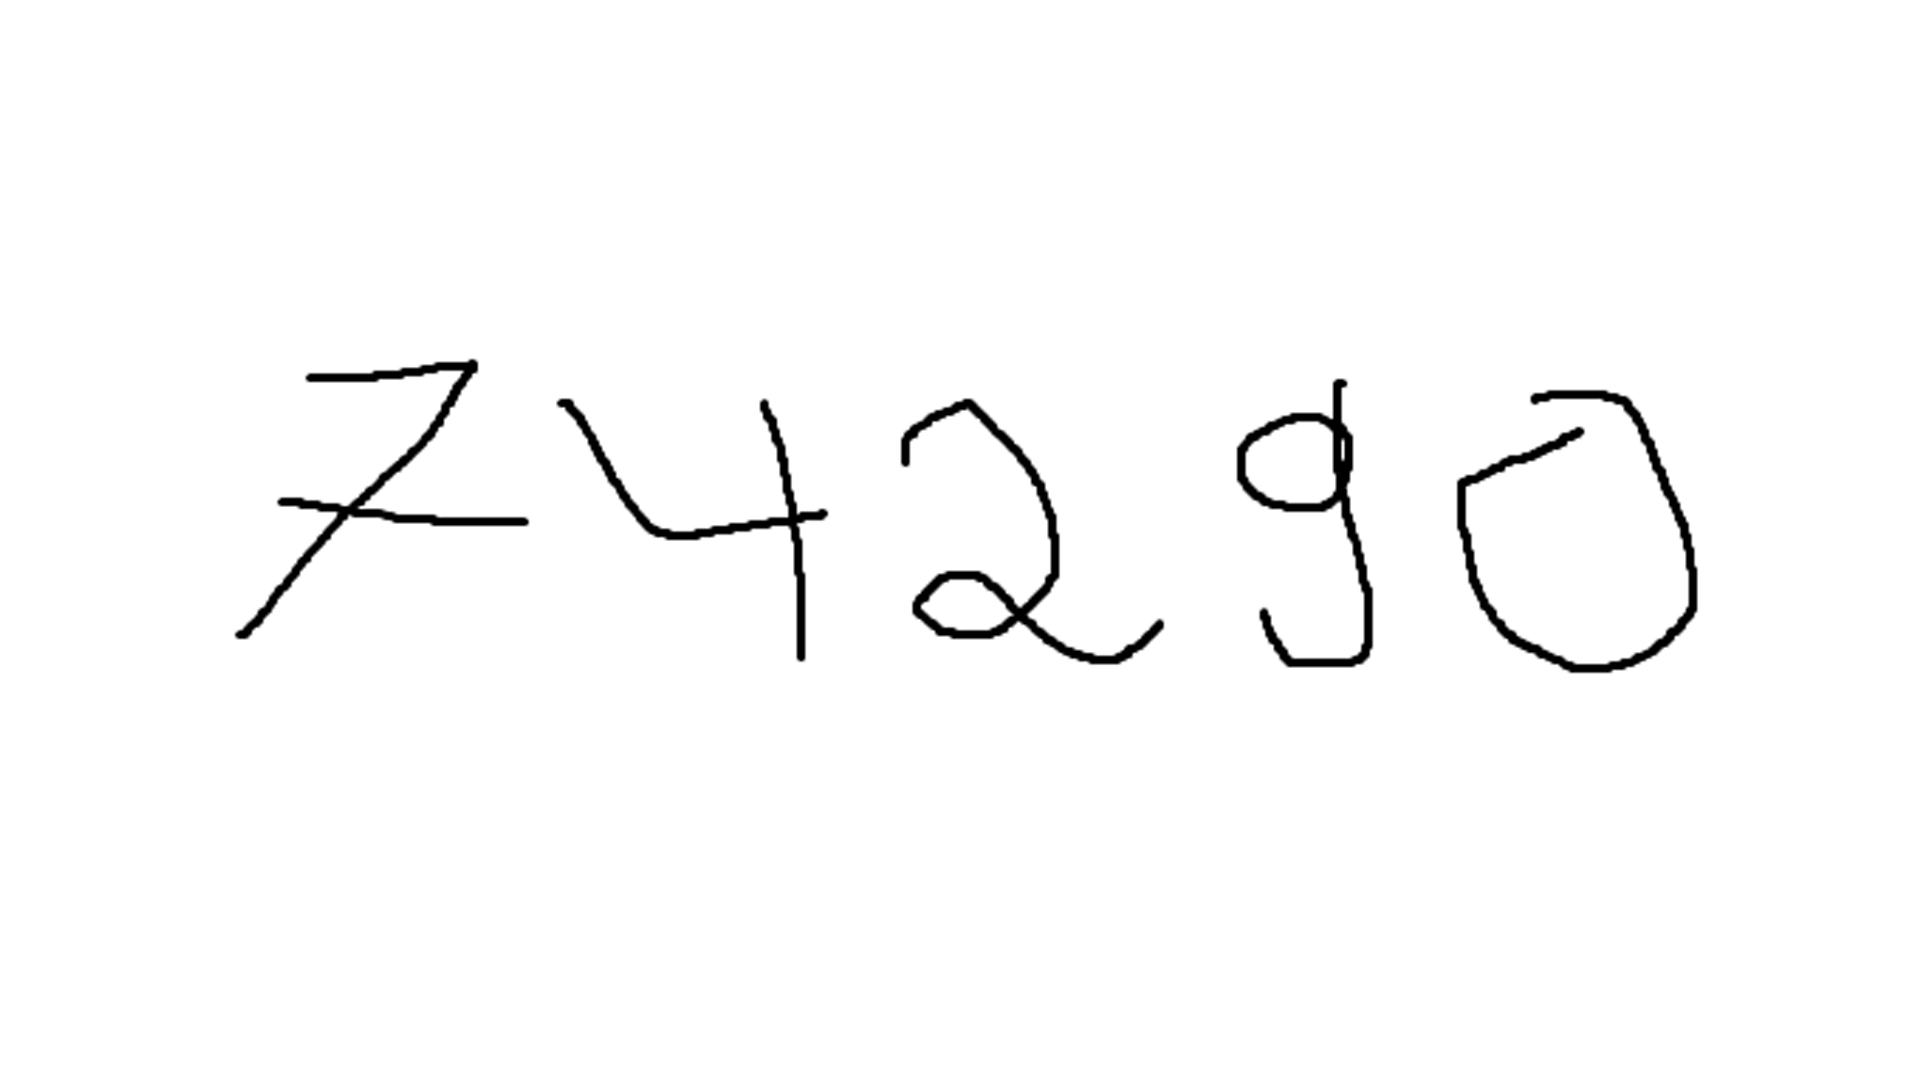
\includegraphics[width=300pt, keepaspectratio]{images/zahlen}
    \caption[Handgeschriebene]{Erkennbar ist die handgeschriebene Zahl 74290.}
\end{figure}
Eine Problemstellung entsteht, wie handgeschriebene Zahlen erkannt werden können.
Dieses Thema ist von besonderem Interesse, weil das Verständnis zur Funktionsweise eines menschlichen Gehirns zum Teil vertieft werden kann.
Außerdem wird die Machenismus eines Textscanners verstanden, was im Alltag von den meisten unbewusst benutzt wird.
Viele Forscher versuchten deshalb in der Vergangenheit nach Problemlösungen zu suchen. Ein Ansatz wäre das Herausfinden
der Strukturen der einzelnen Zahlen und damit die Unterscheidungen zwischen den Zahlen.
Doch jedes Merkmal einer Zahl selber herauszufinden und dann speziell für jede Zahl das zu programmieren kann
anstrengend sein und lange dauern. Mithilfe einer Künstlichen Intelligenz (KI) kann die Erkennung von handgeschriebenen Zahlen ermöglicht werden. 
Schon heute werden KI-Systeme in unseren Alltag integriert, wie zum Beispiel Textübersetzer oder Gesichtserkennung im Smartphone. Da die KI solche
komplexe Strukturen erkennen kann, was ein Mensch vielleicht nicht erkennt, wird die Facharbeit für die Erkennung der handgeschriebenen Zahlen eine KI programmieren. 
Ziel der Facharbeit ist es, eine KI zu programmieren, die handgeschriebene Zahlen mit einer Wahrscheinlichkeit von mindestens 97\% bestimmen zu können.
Auch soll die Möglichkeit bestehen, eigene handgeschriebene Zahlen von der KI testen zu lassen. Um dies umsetzen zu können, wird der Begriff KI definiert und
verschiedene Arten von KIs, welche Funktion jede einzelne Art besitzt, auseinandergesetzt. Die angewendete Lernmethode wird genauer erläutert.
Danach wird in Kapitel 3 über mehrschichtiges Lernen erklärt und Voraussetzungen für diese Methodik genannt. Im Anschluss wird in Kapitel 4
der Aufbau eines faltendes neuronales Netzwerkes dargestellt und die Funktionsweise mathematisch näher gebracht. Dabei wird darauf eingegangen, wie eine KI
lernt und wie sie bestimmte Merkmale der Zahlen erkennen kann mithilfe von 2D Konvolution. Der Begriff Merkmal wird auch in dem Kapitel erläutert.
Mithilfe der Theorie wird dann in Kapitel 5 die KI umgesetzt und programmiert. Dabei wird sie ausgewertet für analysiert, worauf bei der Lernphase
geachtet werden muss. Dies kann durch die Analyse optimiert werden. Zum Schluss wird angeschaut, ob das Ziel der Facharbeit erreicht wurde und welche
Verbesserungsvorschlägen eingefügt werden können, damit die KI eine höhere Wahrscheinlichkeit hat, die Zahl richtig vorherzusagen.
%Gesellschaft.\label{1} Es gibt viele~\cite{useofki}


\section{Künstliche Intelligenz}
Der Begriff Künstliche Intelligenz (KI) ist sehr schwer definierbar, denn es mangelt an der Definition der Bezeichnung Intelligenz.
Allgemein kann die KI definiert werden als der Versuch, bestimmte Entscheidungsstrukturen von Menschen nachzubilden mithilfe von
Algorithmen. Manche Experten behaupten aber auch, dass eine KI nicht gleich eine KI ist, sondern sie in zwei Bereiche unterteilt werden kann.
Dabei wird die KI zwischen einer starke KI und einer schwache KI unterschieden. Schwache KIs sind nur in bestimmten Teilbereichen in der Lage,
an die menschliche Intelligenz heranzukommen. Doch sie ist nicht anpassungsfähig. Das bedeutet, dass eine schwache KI, die zum Beispiel auf Schach
spezialisiert wird, nur die Intelligenz im Bereich Schach besitzt. Selbstständiges Fahren ist mit der KI nicht möglich. Dafür muss eine
andere KI spezialisiert werden, damit sie selbstständig fahren kann. Dagegen kann eine starke KI sich an derzeitigen Situationen anpassen. Diese nennen sich auch Superintelligenz.
Solche starke KIs sind heutzutage noch nicht umsetzbar und es wird schließlich daran geforscht.
Die schwache KI, die in der Facharbeit speziell zur Erkennung von handgeschriebenen Zahlen programmiert wird, können in 2 Teilbereichen
unterteilt werden.
\begin{figure}[h]
    \centering
    \includegraphics[width=300pt, keepaspectratio]{images/ki\_kategorie}
    \caption[Unterkategorien der Künstliche Intelligenz]{Die KI besitzt 2 Unterkategorien, Maschinelles Lernen und Mehrschichtiges Lernen.}
\end{figure}
Eine Unterkategorie der KI wäre der Bereich Maschinelles Lernen. Maschinelles Lernen versucht mithilfe von Algorithmen mit einer großen Anzahl von
Daten ein Muster zu erkennen. Dazu werden die aus der Datens gewonnene Erkenntnisse für Problemlösung verwendet oder der Algorithmus wird auf
die Daten zugeschnitten und verallgemeinert.
Der zweite Teilbereich wäre mehrschichtiges Lernen, das sehr an maschinelles Lernen ähnelt. Der Unterschied liegt aber an der Art und Weise, wie
sie mit den Daten arbeitet. Mehrschichtiges Lernen versucht das menschliche Gehirn zu imitieren durch ein künstliches Neuronales Netzwerk.
Durch das Imitieren sind die Strukturen vom mehrschichtigen Lernen merklich komplexer als die vom maschinellen Lernen. Deswegen sind
sehr große Datensätze von Vorteil für mehrschichtiges Lernen, da deutlich mehr Merkmale der Daten erkannt werden. Darauf basiert sich die KI
in der Facharbeit.
\subsection{Überwachtes Lernen}
Überwachtes Lernen ist eine Methode, wie die KI mit Daten lernen kann. Dazu hat die Datei 2 wichtige Merkmale, nämlich die Eingabe und die
Ausgabe. Die Eingabe wird an die KI zum Lernen geschickt und dabei gibt die KI ein Ergebnis aus. Mit der Ausgabe der Datei wird nun überprüft, ob
die Antwort, die die KI ausgegeben hat, übereinstimmt.
\begin{figure}[h]
    \centering
    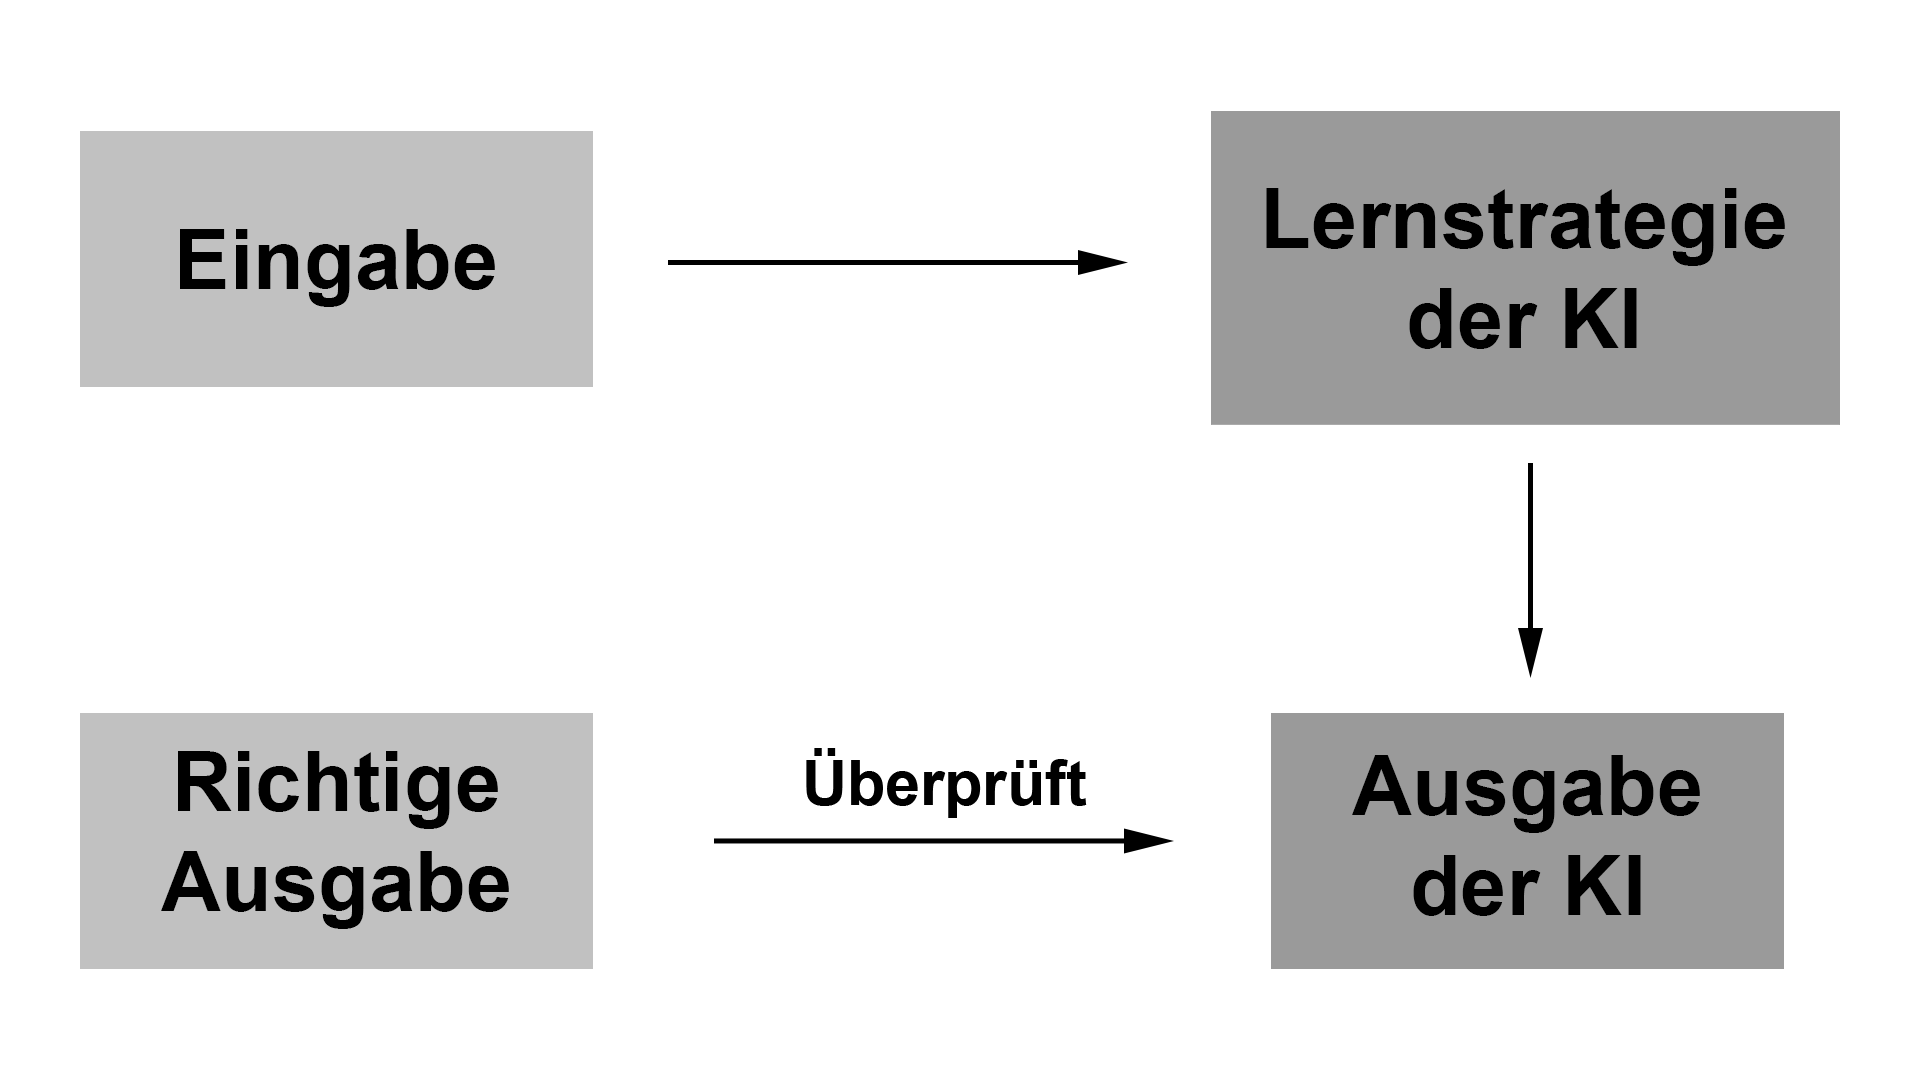
\includegraphics[width=300pt, keepaspectratio]{images/slearning}
    \caption[Ablauf eines überwachtes Lernen]{Zuerst wird die Eingabe verwendet, um zu lernen. Dafür verwendet die KI eine Lernstrategie. Nachdem etwas
    ausgegeben wird, werden die Ausgaben vergliechen.}
\end{figure}
Falls sie nicht übereinstimmt, lernt die KI aus den Fehlern und verbessert sich
dadurch. Überwachtes Lernen ist eine angemessene Methode für das Problem der Facharbeit, da die Antwort, die die KI ausgibt, sich mit der richtigen Antwort decken muss.
Dadurch wird die Fehlerquote der KI möglichst kleingehalten, sodass eine genaue Erkennung der handgeschrieben Zahlen gelingen kann.
Dabei ist anzumerken, dass die KI zwei Arten von Lösungen angeben kann. In dem Fall wird die sogenannte Klassifikation als Lösungsart akzeptiert.
Jede Zahl wird als eine eigene Klasse zugeordnet. Die KI gibt aus, um welche Klasse es sich handelt.

\section{Voraussetzung für mehrschichtiges Lernen}
Im Gegensatz von maschinelles Lernen braucht das mehrschichtige Lernen sehr viele Daten. Es wird von mindestens 10000 Daten gesprochen.
Denn je größer der Datensatz ist, desto besser schneidet mehrschichtiges Lernen ab als maschinelles Lernen. Im Gegenzug verbaucht diese Methode mehr
Rechenleistung. So kann es mehrere Tage oder Wochen dauern, bis die KI fertig gelernt hat und einsatzbereit ist. Auch braucht die KI ein Modell zum
Lernen, ein Künstliches Neuronales Netzwerk. Dafür gibt es verschieden Modelle von Netzwerken. Die Auswahl des Modells für die KI wird später im Kapitel
\nameref{nn} erläutert.

\subsection{Datensatz}
Datensätze sind für die KIs das wichtigste Werkzeug für das Lernen. Denn die Qualität des Datensatzen bestimmt die Lerneffizienz der KI.\@
Je schlechter die Qualität ist, desto schlechter lernt auch die KI.\@ Wichtige Merkmale für Qualität ist die Auflösung, die Anzahl der Daten und die Varibialität.
Für mehrschichtiges Lernen wird ein großer Datensatz gebraucht. Dabei wird für die Problemlösung der MNIST Datensatz von Yann LeCun gewählt.
Sie besitzt insgesamt 70000 Bilder mit handgeschrieben Zahlen, die die Werte zwischen 0 und 9 besitzt. Jedes Bild hat ein 28$\times$28 Pixel
Format und ist farblos. Sie wird nur mit der Hellgikeit dargstellt zwischen 0 und 255. Außerdem hat jedes Bild einen Wert, um welche Zahl
es sich handelt, damit später geprüft werden kann, ob die KI die Zahl richtig erkannt hat oder ob sie falsch liegt.
\begin{figure}[h]
    \centering
    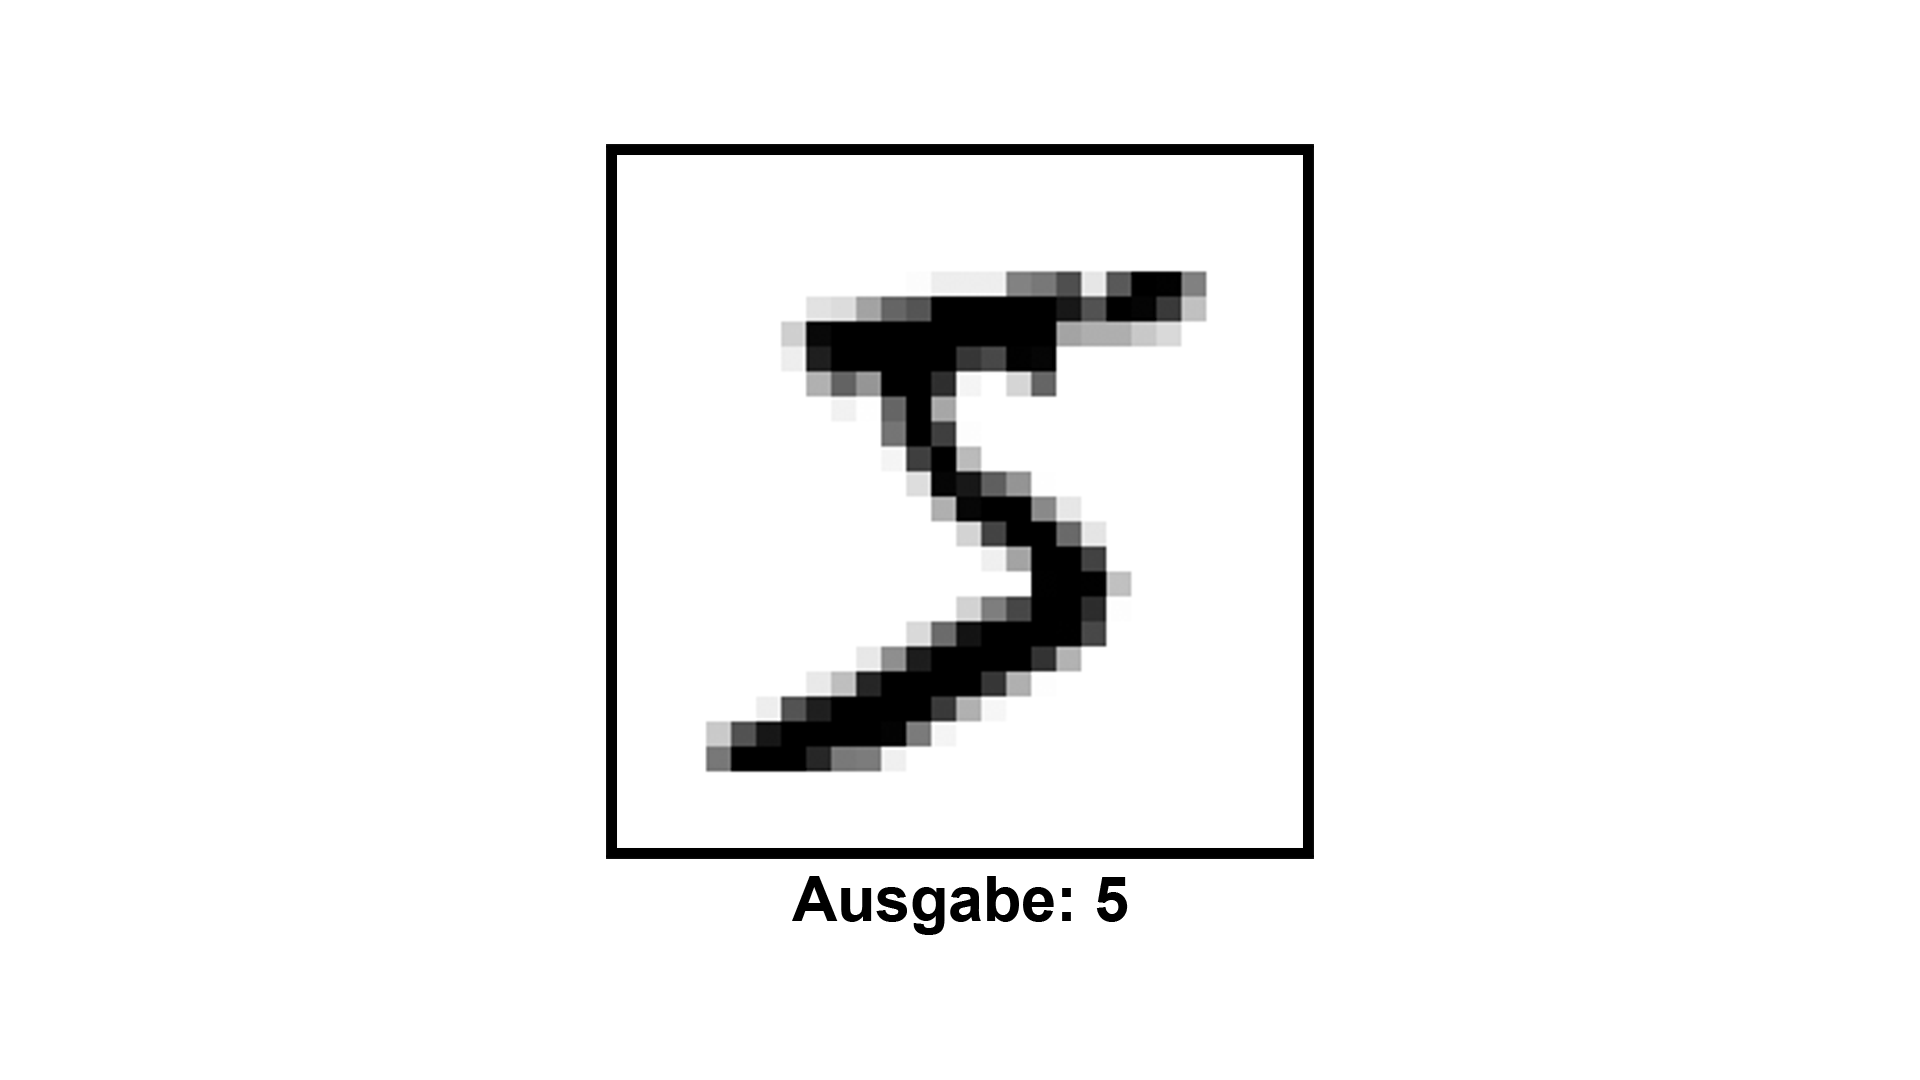
\includegraphics[width=300pt, keepaspectratio]{images/number}
    \caption[Handgeschriebene Zahl 5]{Handgeschriebene Zahl als Abbildung in 28\times28 Pixeln dargestellt, dabei ist die richtige Ausgabe die Zahl 5.}
\end{figure}
Der Datensatz ist gut zum Lernen, denn sie besitzt keine Fehlwerte oder verzerrende Bilder, die die KI beim Lernen stören kann. Auch ist die
Auflösung in Ordnung und 70000 Bilder sind für kleine Aufgaben angemessen.

\subsection{Künstliches neuronales Netzwerk}\label{nn}
Im menschlichen Gehirn befinden sich großen Mengen von Neuronen, die miteinander interagieren. 
Das Neuron besteht aus drei relevante Komponente. Der erste Komponent besteht aus Empfängern, die Signale von anderen verbundeten Neuronen empfängt.
Sie werden auch Dendriten genannt. Ein weiterer Komponent wären die Synapsen. Die Aufgabe ist es sogenannte Neurotransmitter an anderen verbundenen Neuronen
weiterzuleiten, falls das Signal ankommen sollte. Damit das Signal ankommt, braucht es den dritten Komponent, zwar den Axon. Sie wird als Leitungsbahn
verwendet, um Signale transportieren zu können und besteht aus einer lange dünne Röhre. Diese Röhre kann das Signal zu den Synapsen weiterleiten, unter Voraussetzung, dass der Schwellenwert erreicht ist.
Fall er nicht erreicht werden sollte, wird das Signal abgebrochen. Der Schwellenwert wird erreicht, wenn genug Neurotransmitter vorhanden sind.
Sobald das Signal ankommt, werden die Neurotransmitter
ausgeschüttet und die Dendriten der anderen verbunden Neuronen nehmen sie auf.
Dadurch ändert sich die Struktur des Neurons und es kommt wieder zur Entscheidung, ob das Signal weitergeleitet werden soll oder abgebrochen wird.
Es ensteht eine Kettenreaktion.
\begin{figure}[h]
    \centering
    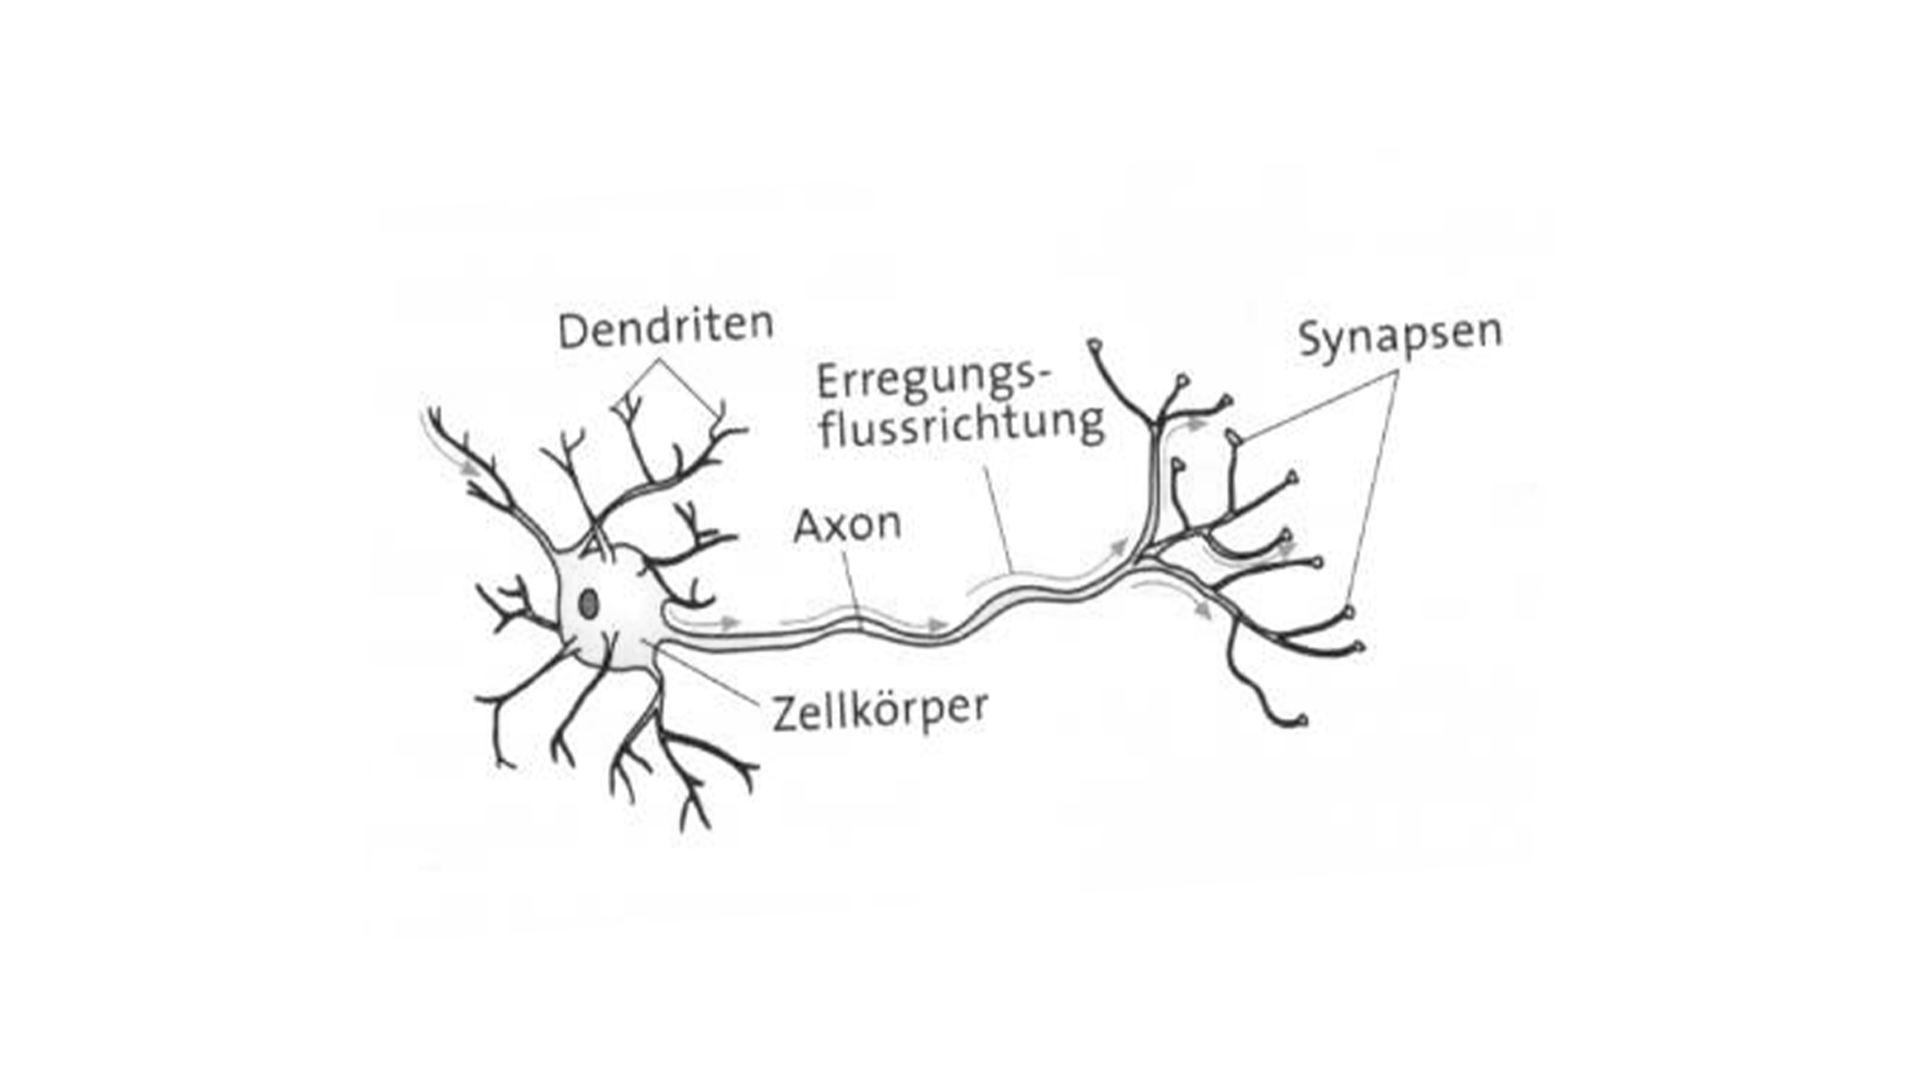
\includegraphics[width=350pt, keepaspectratio]{images/neuron}
    \caption[Aufbau eines Neuron]{Das einzelne Neuron sendet mithilfe der Synapsen Signale an die verbundenen Neuronen, die diese Signale mit den Dendriten aufnehmen.}
\end{figure}
Da das menschliche Gehirn imitiert werden soll, werden künstliche Neuronen erschaffen, die einen Wert von den vorherigen künstlichen Neuronen verarbeitet wurden.
Durch die ganzen Verbindungen zwischen den Neuronen wird das auch als Netzwerk bezeichnet. Viele Eigenschaften der Neuronen werden mitgenommen, wie zum Beispiel die Dendriten, die Synapsen, sowie
der Schwellenwert, in der Informatik auch Bias genannt. Der Bias spielt im Kapitel \nameref{fcnn} eine Rolle. Unterschied ist aber,
dass die künstlichen Neuronen deren Struktur nicht ändern können, dafür können denen aber Werte gegeben werden. Das bedeutet, dass das künstliche Neuron
negative Werte annehmen kann, was bei den Neuronen nicht der Fall ist, da der Axon nur das Signal weiterleiten oder abbrechen kann. Sie können auch mit 0 und 1 bezeichnet werden.
\begin{figure}[h]
    \centering
    \includegraphics[width=300pt, keepaspectratio]{images/neural\_network}
    \caption[Künstliches Neuronales Netzwerk]{Künstliches Neuronales Netzwerk mit insgesamt 37 künstliche Neuronen in 6 Schichten verteilt.}\label{fnnpic}
\end{figure}
Das Netzwerk kann unterschiedliche Anordnungen von künstlichen Neuronen besitzen. Die geeignetste Anordnung nennt sich das
konvolutionales neuronales Netzwerk (CNN), denn sie wird häufig für Bildererkennung verwendet. Grund dafür ist die Extrahierung der Merkmale
des Bildes. Denn bevor das Bild an die künstlichen Neuronen weitergeleitet werden, werden unnötige Merkmale mithilfe von Konvolution aus dem Bild entfernt, sodass der
Lernprozess der KI auf das Wichtigste begrenzt wird. Welche Merkmale eines Bildes gemeint ist, wird im Kapitel \nameref{feature} verdeutlicht.

\section{Konvolutionales neuronales Netzwerk}

Das CNN kann in zwei Bereichen gegliedert werden. Im ersten Bereich werden Merkmale des Bildes extrahiert, wie zum Beispiel Ecken, Kurven, etc. Diese nennt sich Feature Extraction.
Die Extrahierung wird durch 2D Convolution berechnet. Im zweiten Bereich werden die
wichtigen Merkmalen aus der Feature Extraction in die sogenannte Klassifikationsebene weitergeleitet. Dort fängt der Lernprozess
der KI an, die dann am Ende des Netzwerkes eine Klasse ausgibt.

\subsection{Klassifikationsebene}\label{fcnn}
In der Klassifikationsebene befindet sich das künstliches neuronales Netzwerk, die eine ähnliche Struktur wie bei Abbildung~\ref{fnnpic} hat.
Diese Struktur nennt sich auch Vorwärtsgerichtetes Neuronales Netzwerk (FNN) und ist in mehreren Schichten aufgebaut. In Abbildung~\ref{fnnpic} wäre die Anzahl
der Schichten $A = 6$. Die erste Schicht nennt sich Eingabeschicht, denn von dort kommen die Daten in die Neuronen rein, während bei
der letzte Schicht die KI ein Ergebnis ausgibt. Diese Schicht heißt Ausgabeschicht. Die Schichten dazwischen werden ausgeblendete Schichten genannt.
Die ausgeblendete Schichten sind wichtige Teile des Netzwerkes, denn durch diese werden Merkmale gesucht und analysiert.
Das Netzwerk läuft also von links nach rechts durch. Das gibt nochmal
eine deutlich stärkere Lerntiefe für die KI.\@ Die einzelne Neuronen können einen Wert besitzen, sie wird als $ x_{i}^{(\alpha,\beta)} $ definiert,
wobei $ \alpha \in \{1,\ldots,A\} $ gilt. Der Index $i$ beschreibt um welches Neuron in der Schicht $\alpha$ es sich handelt. Der Wert $\beta$ wird später
verwendet. Für die Einheitlichkeit der Formeln steht in dem Fall $\beta$ in der Variable. In der Klassifikationsebene bleibt $\beta = 1$. Dieser Wert
lässt sich aus den ganzen Verbindungen der vorherigen Schicht berechnen, indem sie wie in Abbildung~\ref{connection} addiert werden. Dabei werden
die einzelne Werte $ x_{j}^{(\alpha-1,1)} $ mit einem Gewicht $ w_{i,j}^{(\alpha,1)} $ multipliziert, womit $ j \in \{1,\ldots,N_{\alpha-1}\} $ gilt.
$ N_{\alpha} $ beschreibt die Anzahl der Neuronen auf der Schicht $\alpha$.
\begin{figure}[h]
    \centering
    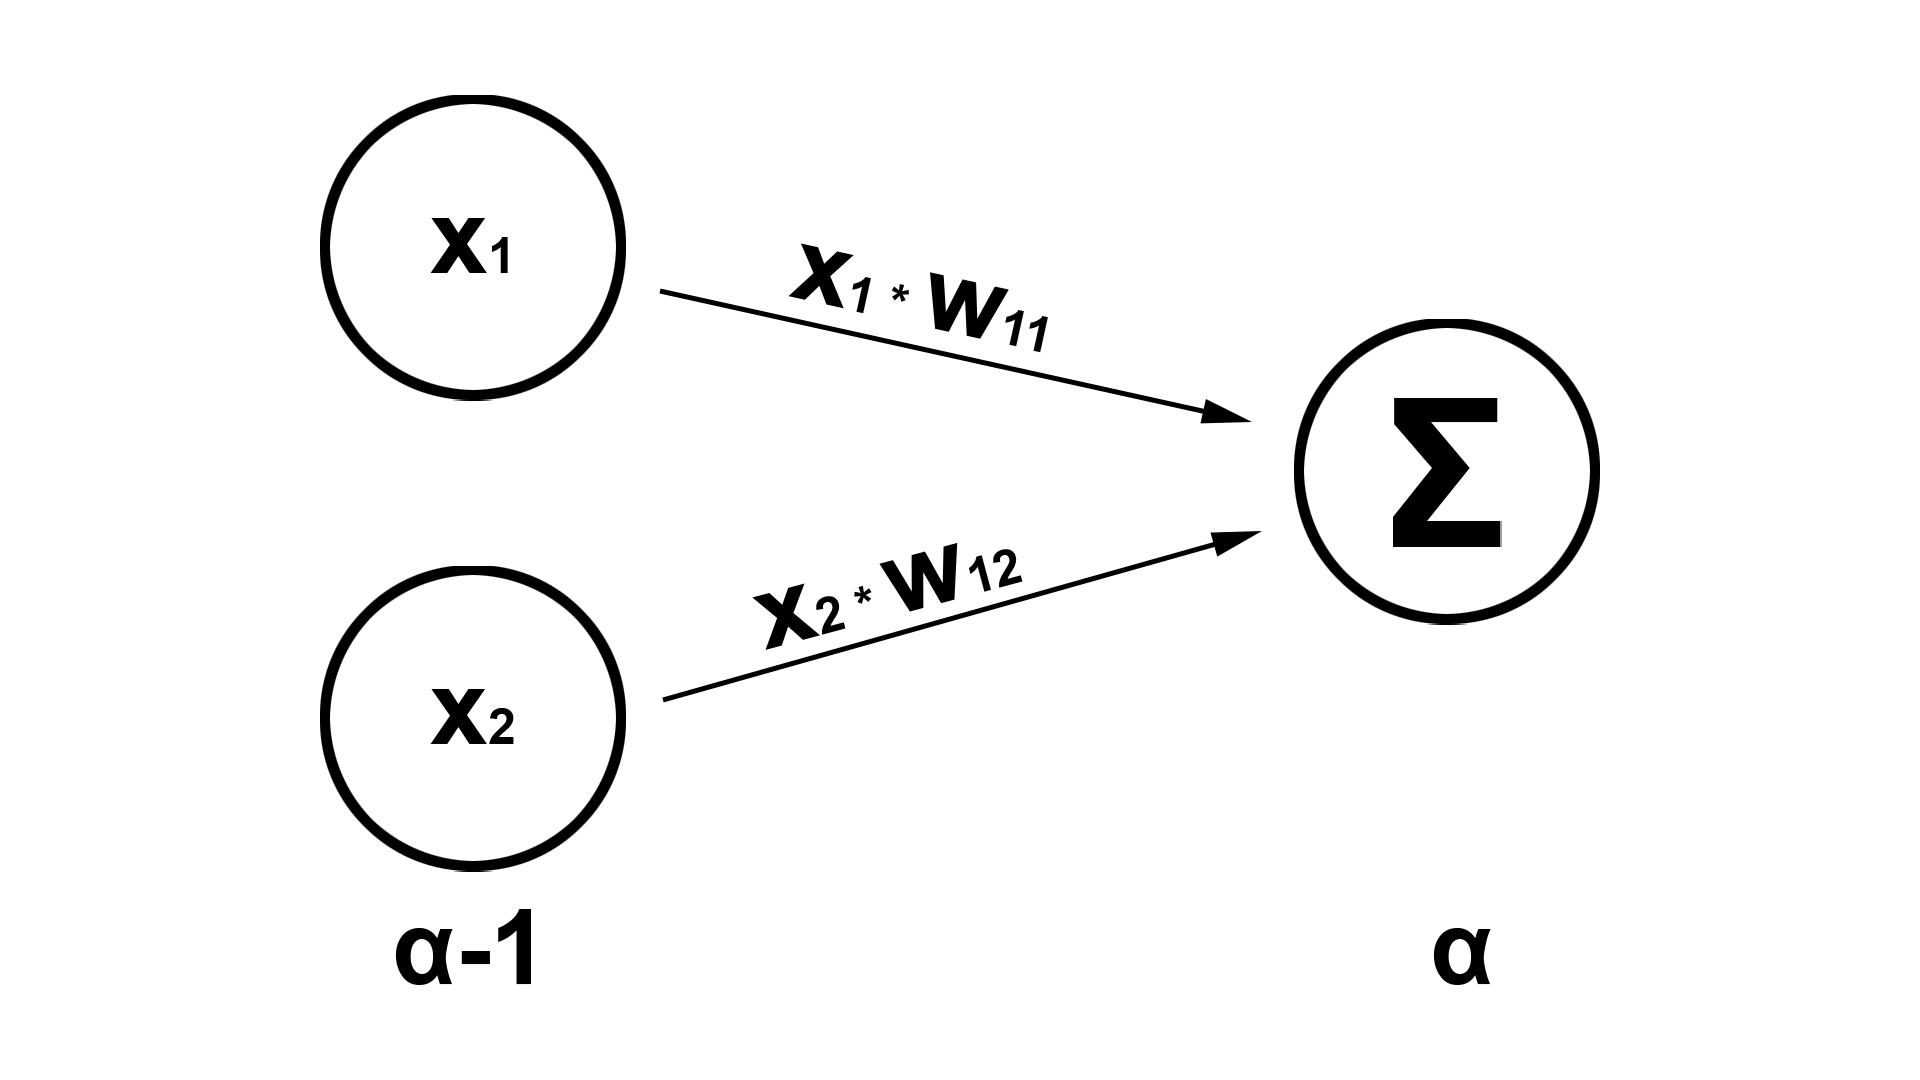
\includegraphics[width=300pt, keepaspectratio]{images/verbindung}
    \caption[Verbindungen zwischen den Neuronen]{Die Verbindungen zwischen den Neuronen werden mit den Parameter $w$ erweitert.}\label{connection}
\end{figure}
Allgemein gilt dann für die Berechnung
\begin{equation}
    \label{xwithoutfunction}
    \bar{x}_{i}^{(\alpha,1)} := \sum_{j=1}^{N_{\alpha-1}} w_{i,j}^{(\alpha,1)} x_{j}^{(\alpha-1,1)} + b_{i}^{(\alpha,1)} \quad i \in \{1,\ldots,N_{\alpha}\}, j \in \{1,\ldots,N_{\alpha-1}\}.
\end{equation}
Das $ b_{i}^{(\alpha,1)} $ in der Gleichung steht für Bias und ist ein weiterer Parameter zum Einstellen wie das Gewicht. Beide spielen hier eine wichtige Rolle
für das Weiterleiten der Neuronen. Das Gewicht entscheidet, wie wichtig der Wert vom Neuron ist. Je höher der Wert ist, desto entscheidener
ist das Neuron. Wichtig ist anzumerken, dass die Gewichte und die Biases verstellbare Parameter sind, die für das Lernen der KI eine wichtige Rolle
spielt. Damit die KI lernen kann, müssen die Parameter $w$ und $b$ optimal gesetzt werden, sodass die KI richtige Voraussagen treffen kann, um welche Zahl es sich handelt.
Dafür wird die Fehlerzurückführung (Backpropagation) verwendet. Erstmal werden nur die partielle Ableitungen berechnet. Warum sie gebraucht werden wird im Kapitel \nameref{back} genauer
erläutert. So kann in der Gleichung~\ref{xwithoutfunction} partiell nach drei Variablen der Funktion $C(\vec{y},\vec{x}^{(A,1)})$ abgeleitet werden: $x_{j}^{(\alpha-1,1)}$, $w_{i,j}^{(\alpha,1)}$ und $b_{i}^{(\alpha,1)}$.
Auch die Funktion $C(\vec{y},\vec{x}^{(A,1)})$ wird in Kaptiel \nameref{lost} genauer erläutert.
Folgendes ergibt sich:
\begin{equation}
    \frac{\partial C}{\partial b_i^{(\alpha,1)}} = \frac{\partial C}{\partial \bar{x}_i^{(\alpha,1)}}
\end{equation}
\begin{equation}
    \frac{\partial C}{\partial w_{i,j}^{(\alpha,1)}} = \frac{\partial C}{\partial \bar{x}_i^{(\alpha,1)}} x_j^{(\alpha-1,1)}
    \label{w}
\end{equation}
\begin{equation}
    \frac{\partial C}{\partial x_{j}^{(\alpha-1,1)}} = \sum_{i=1}^{N_{\alpha}} \frac{\partial C}{\partial \bar{x}_i^{(\alpha,1)}} w_{i,j}^{(\alpha,1)}
\end{equation}
Eine weitere Sache, die hinzugefügt werden muss, ist die Aktivierungsfunktion, denn sie gibt das Netzwerk eine Komplexität.
Ohne diese Komplexität wäre das Netzwerk linear, was Nachteile mit sich bringt für die KI. In Abbildung~\ref{regressionpic} ist die Regression bei einer
nicht lineare Struktur deutlich besser als dies einer lineare Struktur.
\begin{figure}[h]
    \centering
    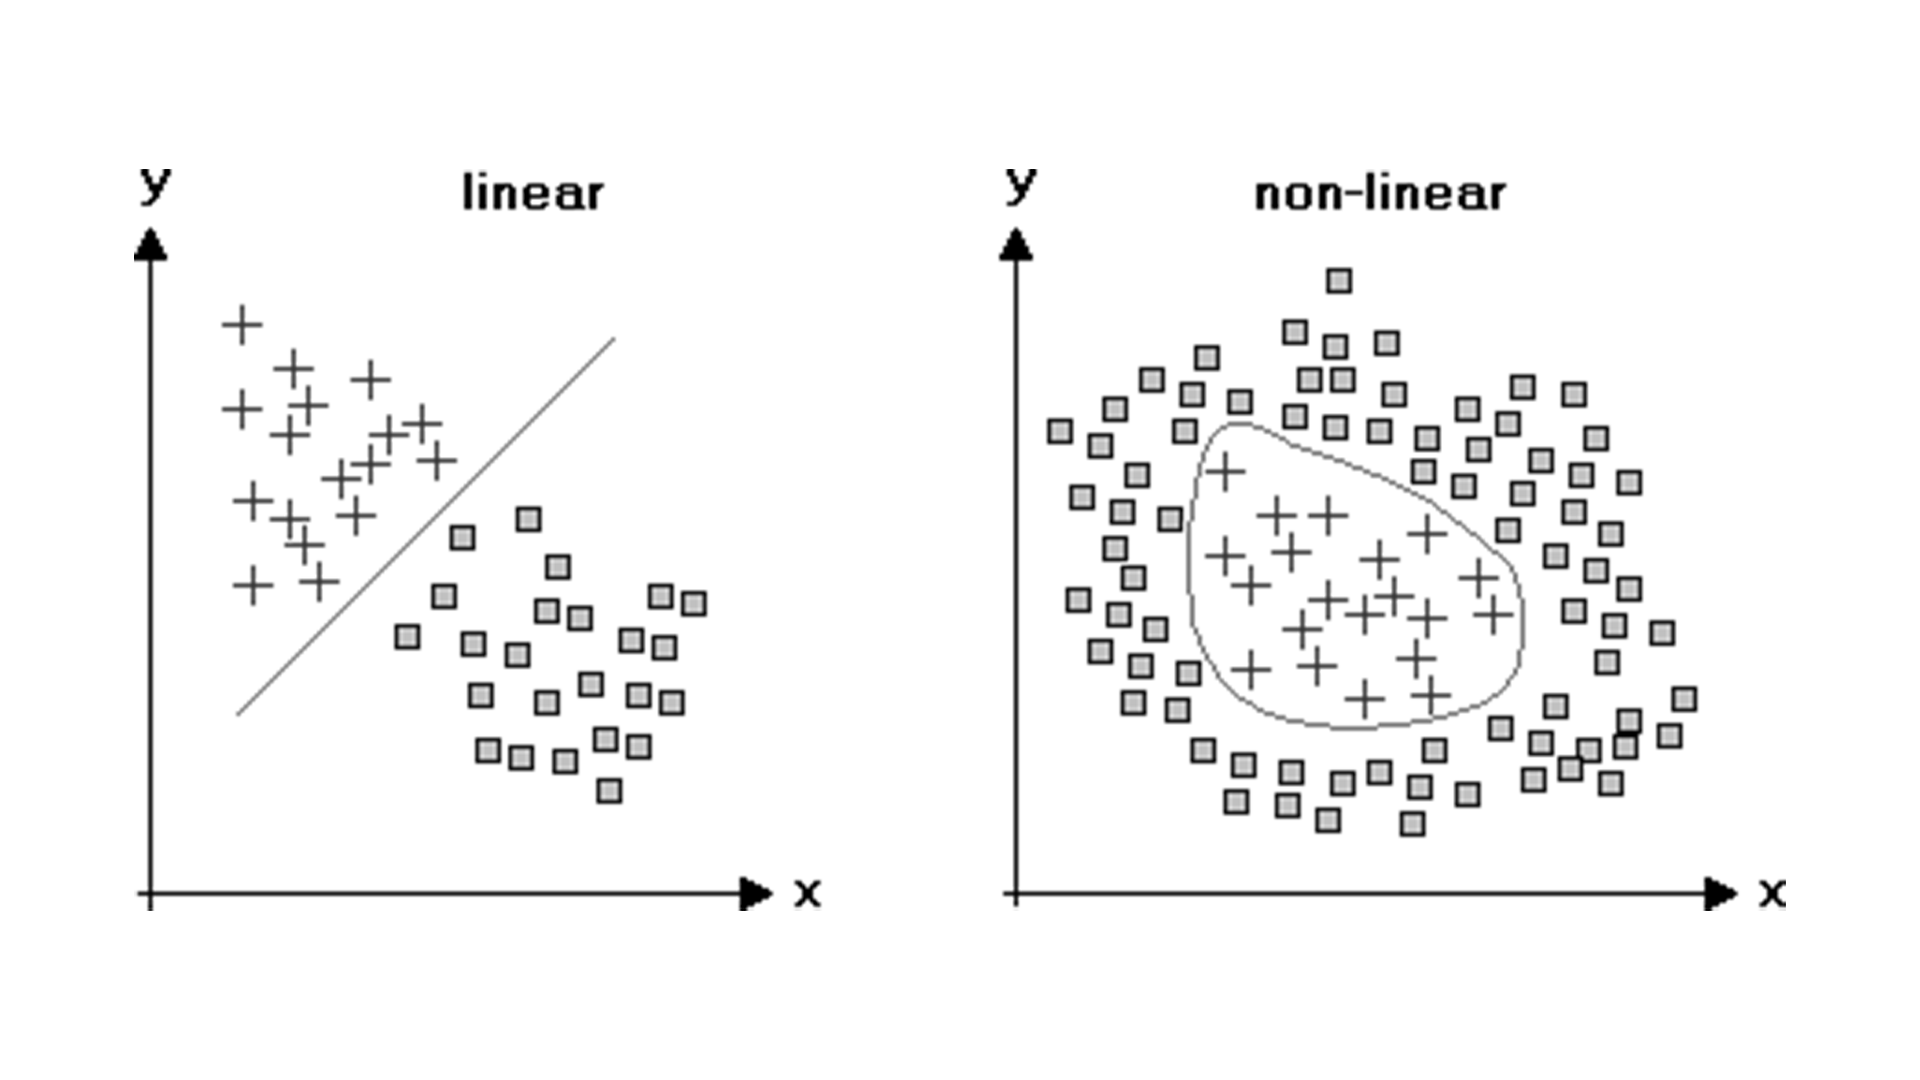
\includegraphics[width=300pt, keepaspectratio]{images/regression}
    \caption[Lineare Regression und nicht lineare Regression]{Im ersten Graph ist sie gut mit der lineare Regressionen lösbar. Beim zweiten Graph ist es
    unmöglich eine genaue Regression zu bekommen mit einer lineare Regression. Dafür wird eine nicht linieare Regression verwendet.}\label{regressionpic}
\end{figure}
Welche Aktivierungsfunktionen verwendet werden kommt im Kapitel \nameref{activation} dran. So ergibt sich
\begin{equation}
    x_{i}^{(\alpha,1)} := f^{(\alpha,1)}(\bar{x}_{i}^{(\alpha,1)}) = f^{(\alpha,1)}(\sum_{j=1}^{N_{\alpha}} w_{i,j}^{(\alpha,1)} x_{j}^{(\alpha-1,1)} + b_{i}^{(\alpha,1)}).
\end{equation}
Nun kann die Schicht auch als einen Vektor angesehen werden, wobei die Neuronen die Elemente vom Vektor sind. Folglich kann das Netzwerk
in Abbildung~\ref{fnnpic} in einem Matrixblock umgeschrieben werden. So definiert sich
\begin{equation}\label{withfunction}
    \vec{x}^{(\alpha,1)} := \begin{bmatrix}x_{1}^{(\alpha,1)} \\ x_{2}^{(\alpha,1)} \\ \ldots \\ x_{N_{\alpha}}^{(\alpha,1)} \end{bmatrix}.
\end{equation}
Sobald die letzte Schicht erreicht ist, berechnet die Verlustfunktion Fehlermaße des Netzwerkes und gibt Aussage darüber, wie gut
unsere KI ist. Mehr dazu im Kapitel \nameref{lost}.


\subsubsection{Aktivierungsfunktion}\label{activation}
Mithilfe der Aktivierungsfunktion kann die KI eine nicht lineare Regression durchführen, denn aus der Gleichung~\ref{withfunction} wird deutlich,
dass alle Operationen linear sind, wenn nur der Paramater der Funktion $f^{(\alpha,1)}(x)$ betrachtet wird. Für eine nicht lineare Regression sollte die
Aktivierungsfunktion differenzierbar sein. Dafür gibt es verschiedene Formen von Aktivierungsfunktionen, die in der Praxis angewendet werden.
Eine der meist verwendeten Aktivierungsfunktionen ist der Rectified linear unit (ReLU):
\begin{equation}
    f^{(\alpha,1)}(\bar{x}_{i}^{(\alpha,1)}) = \left\{
	\begin{array}{ll}
		\bar{x}_i^{(\alpha,1)}  & \mathrm{falls} \mkern5mu \bar{x}_i^{(\alpha,1)} > 0 \\
		0 & \mathrm{falls} \mkern5mu \bar{x}_i^{(\alpha,1)} \leq 0
	\end{array}
    \right.
\end{equation}
Die partielle Ableitung nach $\bar{x}_i^{(\alpha,1)}$ zur Funktion $C(\vec{y},\vec{x}^{(A,1)})$ ist:
\begin{equation}
    \frac{\partial C}{\partial \bar{x}_i^{(\alpha,1)}} = \left\{
	\begin{array}{ll}
		\frac{\partial C}{\partial {x}_i^{(\alpha,1)}}  & \mathrm{falls} \mkern5mu \bar{x}_i^{(\alpha,1)} > 0 \\
		0 & \mathrm{falls} \mkern5mu \bar{x}_i^{'(\alpha,1)} \leq 0
	\end{array}
    \right.
\end{equation}
Gründe für die Nutzung ist die Effizienz für linear gebaute Neuronale Netzwerke, sowie die Berechnung der Werte. Außerdem kann durch ReLU
Neuronen dauerhaft deaktiviert werden, da alle Werte, die $\leq 0$ sind, zu $0$ gesetzt werden.
Die Ableitungs
Eine weitere Aktivierungsfunktion, die für die Facharbeit verwendet wird ist die Softmax Funktion:
\begin{equation}\label{softmax}
    f^{(\alpha,1)}(\bar{x}_{i}^{(\alpha,1)}) = \frac{e^{\bar{x}_i^{(\alpha,1)}}}{\sum_{j=1}^{N_{\alpha}} e^{\bar{x}_i^{(\alpha,1)}}}
\end{equation}
Die partielle Ableitung nach $\bar{x}_i^{(\alpha,1)}$ zur Funktion $C(\vec{y},\vec{x}^{(A,1)})$ ist:
\begin{equation}
    \frac{\partial C}{\partial \bar{x}_k^{(\alpha,1)}} = \frac{\partial C}{\partial {x}_i^{(\alpha,1)}} (\delta_{i,k}x_{i}^{(\alpha,1)}-x_{i}^{(\alpha,1)}x_{k}^{(\alpha,1)})
\end{equation}
Meistens wird die Aktivierungsfunktion an der letzte Schicht verwendet, denn der Zweck dieser Aktivierungsfunktion ist es mithilfe des Vektors
$ \vec{x}^{(A)} $ in einen neuen Vektor gleicher Dimension zu erstellen, deren Elemente zusammenaddiert $1$ ergibt. Der Wertebereich der Funktion
liegt bei $[0;1]$. Dies kann dann in einer Wahrscheinlichkeitsverteilung dargestellt werden. Dies erleichtert die Dokumentierung der Ergebnisse der KI
und eine Rückschlussziehung, warum die KI wahrscheinlich diese Zahl nimmt, ist möglich.


\subsection{Feature Extraction}\label{feature}
Die Feature Extraction besteht aus mehreren Schichten von Operationen mit dem das eingebene Bild verarbeitet wird.
Eine Hauptoperation ist der 2D Konvolution, denn diese Operation ist dafür zuständig, dass wichtige Merkmale extrahiert werden.
Dafür werden verschiedene Filter angewendet, um verschiedene Arten von Merkmalen des Bilder zu extrahieren.
\begin{figure}[h]
    \centering
    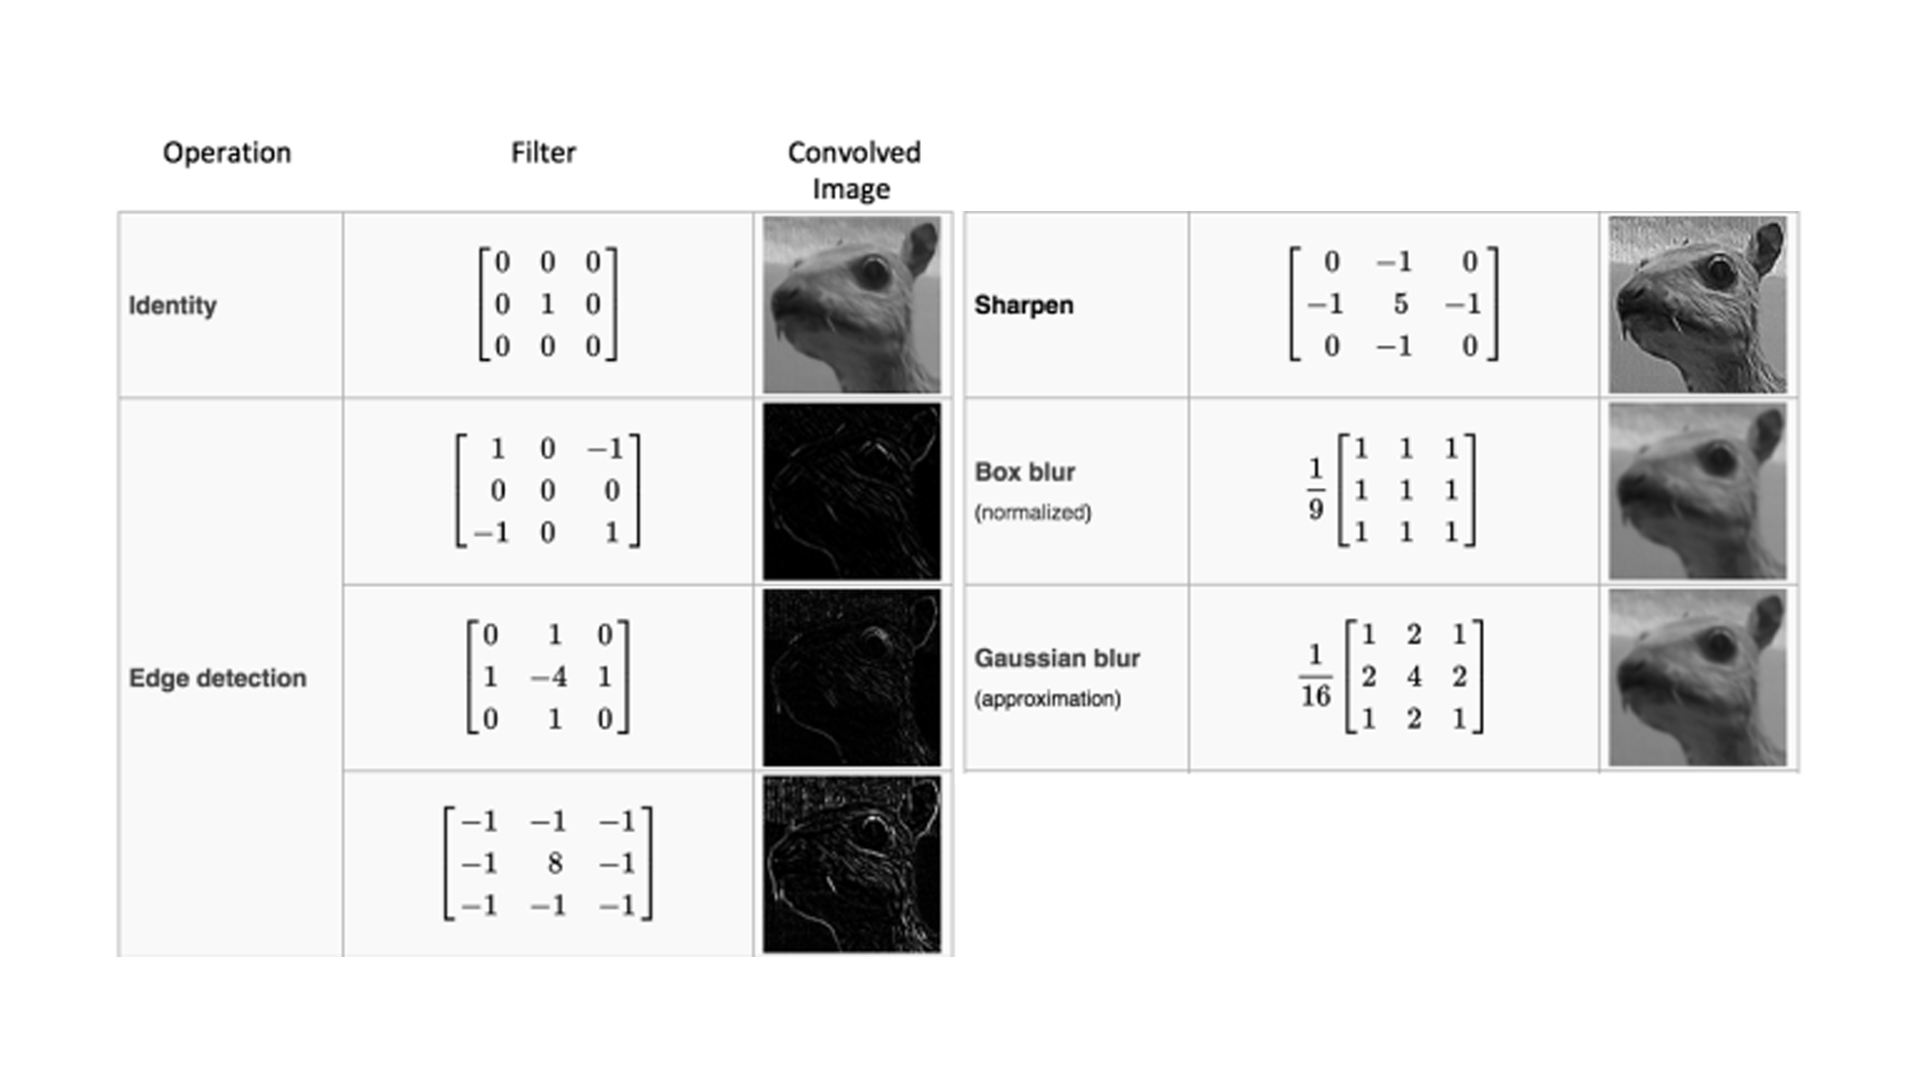
\includegraphics[width=400pt, keepaspectratio]{images/filter}
    \caption[Verschiedene Extraktionsmöglichkeiten]{Hier sind verschiedene Extrahierungen zu erkennen mit verschiedenen Aufgaben. Das erste Bild mit der Operation Identity ist das Originalbild.}\label{kernel}
\end{figure}
Weitere wichtige Operationen ist der Max-Pooling und der Flattening. Aufgabe von Max-Pooling ist es unnötige Merkmale
zu ignorieren, indem nur die hellsten Pixel rausgefiltert werden. Die Dimension des Bildes halbiert sich. Flattening ist für die Übertragung auf die Klassifikationseben zuständig,
indem die Matrix des Bildes in einen Vektor geflacht wird, sodass die KI optimal lernen kann.
Das Bild kann in einer 28\times28 Matrix dargestellt werden
\begin{equation}
    X^{(1,1)} := (x_{ij}) \quad i \in \{1,\ldots,28\}, j \in \{1,\ldots,28\}.
\end{equation}
Der erste Index beschreibt auf welcher Schicht die Variable sich befindet und der zweite Index beschreibt auf welches
Bild sie drauf bezieht, denn in einer Schicht können mehrere Bilder vorkommen. Dies nennt sich Tiefe. Da am Anfang aber nur ein Bild eingegeben wird, gilt
$N_{\beta}^{(1)} = 1$. Für die nächsten Schichten gilt im Allgemeinen
\begin{equation}\label{newlayer}
    X^{(\alpha,\beta)} := (x_{ij}) \quad i \in \{1,\ldots,m_{x}^{(\alpha,\beta)}\}, j \in \{1,\ldots,n_{x}^{(\alpha,\beta)}\}.
\end{equation}
Die Werte $m_{x}^{(\alpha,\beta)}$ und $n_{x}^{(\alpha,\beta)}$ werden basiert auf die Operation berechnet, wobei
$\alpha \in \{1,\ldots,A\}$ und $\beta \in \{1^{(\alpha)},\ldots,N_{\beta}^{(\alpha)}\}$. Dabei ist die Anzahl der Tiefe von der jeweilige Schicht abhängig.


\subsubsection{2D Konvolution}
Mithilfe von 2D Konvolution können wichtige Merkmale herausgefiltert werden. Damit sie aber herausgefiltert werden kann, wird
eine neue Matrix definiert, die auch als Kernel genannt wird
\begin{equation}
    K^{(\alpha,\beta)}:={(k_{i,j})}^{(\alpha,\beta)} \quad i \in\{1;2;\ldots;m_{k}^{(\alpha,\beta)}\}, j \in\{1;2;\ldots;n_{k}^{(\alpha,\beta)}\}
\end{equation}
Der Kernel kann nach der Abbildung~\ref{kernel} verschiedene Formen von Matritzen annehmen, dadurch entsteht durch die 2D Konvolution eine neue Matrix, in dem Fall ein neues Bild
Diese neue Matrix gilt für die nächste Schicht, weshalb die neue Matrix der Gleichung~\ref{newlayer} entspricht, wobei $ m_x \leftarrow m_x - m_k + 1 $ und $ n_x \leftarrow n_x - n_k + 1 $
Da sowohl die Eingabe des Bildes, sowie der Kernel beide Matritzen sind, kann mit der 2D Konvolution gerechnet werden. Sie ist
folgendermaßen defininiert
\begin{equation}
    a_{i,j} = {(X \ast K)}_{i,j} := \sum_{m'=1}^{m_{k}} \sum_{n'=1}^{n_{k}} x_{i-m'+1,j-n'+1}k_{m',n'}. \label{Conv}
\end{equation}
Eine weitere Operation, die sehr wichtig für die 2D Konvolution ist die Kreuzkorrelation (Cross Correlation)
\begin{equation}
    a_{i,j} = {(X \star K)}_{i,j} := \sum_{m'=1}^{m_{k}} \sum_{n'=1}^{n_{k}} x_{i+m'-1,j+n'-1}k_{m',n'}.
\end{equation}
Aus~\eqref{Conv} wird deutlich, dass Cross Correlation nichts anderes ist als eine 2D Konvolution, wo nur der Kernel um 180$^{\circ}$
rotiert ist. Für die Operation können auch Biases, sowie Aktivierungsfunktionen angewandt werden. Dies ähnelt der Struktur der FNN.\@
Werden diese Eigenschaften hinzugefügt, folgt daraus für die 2D Convolution:
\begin{equation}
    x_{i,j}^{(\alpha,\beta)} = f^{(\alpha)}(\sum_{\beta'=1}^{N_{\beta}^{(\alpha-1)}} \sum_{m'=1}^{m_{k}} \sum_{n'=1}^{n_{k}} x_{i+m'-1,j+n'-1}^{(\alpha-1,\beta')}k_{m',n'}^{(\alpha,\beta')}+b_{i,j}^{(\alpha,\beta)})
\end{equation}
Für die Backpropagation werden die partielle Ableitungen nach $k_{i,j}^{(\alpha,\beta)}$, nach $b_{i,j}^{(\alpha,\beta)}$ und nach $x_{i,j}^{(\alpha-1,\beta)}$ zur Funktion $C$ gebraucht:
\begin{equation}
    \frac{\partial C}{\partial k_{i,j}^{(\alpha,\beta)}} = \sum_{i'=1}^{m_x^{(\alpha,\beta)}}\sum_{j'=1}^{n_x^{(\alpha,\beta)}} \frac{\partial C}{\partial \bar{x}_{i',j'}^{(\alpha,\beta)}}
    x_{i+i'-1,j+j'-1}^{(\alpha-1,\beta)} = {(X^{(\alpha-1,\beta)} \star \frac{\partial C}{\partial \bar{X}^{(\alpha,\beta)}})}_{i,j}
\end{equation}
\begin{equation}
    \frac{\partial C}{\partial b_{i,j}^{(\alpha,\beta)}} = \frac{\partial C}{\partial \bar{x}_{i,j}^{(\alpha,\beta)}}
\end{equation}
\begin{equation}
    \frac{\partial C}{\partial x_{i,j}^{(\alpha-1,\beta)}} = \sum_{i'=1}^{m_x^{(\alpha,\beta)}}\sum_{j'=1}^{n_x^{(\alpha,\beta)}} \frac{\partial C}{\partial \bar{x}_{i',j'}^{(\alpha,\beta)}} k_{i-i'+1,j-j'+1}^{(\alpha,\beta)}
    = {(K^{(\alpha,\beta)} \ast \frac{\partial C}{\partial \bar{X}^{(\alpha,\beta)}})}_{i,j}
\end{equation}

\subsubsection{Max-Pooling}
Diese Operationen wird für das CNN öfters benutzt, denn zum einen reduziert sie Bildgröße um die Häflte und zum anderen behält sie trotzdem wichtige
Merkmale des Bildes. Das macht das Berechnen nochmal effizienter und die Hauptmerkmale werden herausgestochen. Dies funktioniert, indem eine 2$\times$2 Matrix
durch die einzelne Regionen des Bildes durchgegangen wird und der höchste Wert von den 4 Pixel ausgewählt wird:
\begin{equation}
    x_{i,j}^{(\alpha,\beta)} = \max\{x_{i',j'}^{(\alpha-1,\beta)} \mkern5mu | \mkern5mu i' \in \{i,i+1\}, j' \in \{j,j+1\} \}.
\end{equation}
Die neue Dimension beträgt
\begin{equation}
    m_{x}^{(\alpha,\beta)} = \bigg\lceil \frac{m_{x}^{(\alpha-1,\beta)}}{2} \bigg\rceil, \mkern5mu
    n_{x}^{(\alpha,\beta)} = \bigg\lceil \frac{n_{x}^{(\alpha-1,\beta)}}{2} \bigg\rceil.
\end{equation}
Bei der Backpropagation ist der Wert der Verlustfunktion nur von den größten Werten der einzelne Regionen abhängig, da nur diese an der nächsten Schicht weitergegeben wurden.
Die anderen Werte spielen keine Rolle, deswegen ist der Gradient von denen = 0.
\begin{equation}
    \frac{\partial C}{\partial x_{i,j}^{(\alpha-1,\beta)}} =
    \left\{
    \begin{array}{ll}
		\frac{\partial C}{\partial \bar{x}_{i,j}^{(\alpha,\beta)}} & \mathrm{falls} \mkern5mu \max\{x_{i',j'}^{(\alpha-1,\beta)} \mkern5mu | \mkern5mu i' \in \{i,i+1\}, j' \in \{j,j+1\} \} \\
		0 & \mathrm{falls} \mkern9mu \mathrm{Sonstiges}
	\end{array}
    \right.
\end{equation}

\subsubsection{Übergang von Feature Extraction zu Klassifikationsebene}
Nachdem die Merkmale der Bilder durch 2D Konvolution und Max-Pooling extrahiert wurden, muss diese Matrix zur Klassifikationsebene übertragen werden.
Da aber die Klassifikationsebene nur einen Vektor als Eingabe annimmt, muss die Matrix abgeflacht werden. Mithilfe des Vektoroperators $vec()$ kann die
Ausgangsmatrix der Feature Extraction in einen Vektor umgewandelt werden:
\begin{equation}
    \vec{x}^{(\alpha,\beta)} = vec_{n_{x}^{(\alpha,\beta)}, m_{x}^{(\alpha,\beta)}}(X^{(\alpha-1,\beta)T})
\end{equation}
Dabei gibt die Indizes die die Dimension der Matrix an, die abgeflacht werden soll. Für die Backpropagation muss der Vektor aber wieder in einer Matrix mit
der gleichen Dimension umgeformt werden. Dafür existiert eine Umkehrfunktion des Vektoroperators $vec^{-1}()$ die diese Berechnung durchführen kann:
\begin{equation}
    X^{(\alpha-1,\beta)} = vec^{-1}_{n_{x}^{(\alpha,\beta)}, m_{x}^{(\alpha,\beta)}}{(\vec{x}^{(\alpha,\beta)})}^{T}
\end{equation}
Dieser Übergang wird auch als Flattening benannt.

\subsection{Verlustfunktion}\label{lost}
Um auszuwerten, ob eine KI gute oder schlechte Vorhersagen trifft, werden Verlustfunktionen verwendet. Verlustfunktionen sind Funktionen, die Abweichungen
der vorhergesagte Zahl $\vec{x}^{(A,1)}$ mit der Ausgangszahl $\vec{y}$ berechnet wird. Je größer die Abweichung ist, desto unpräziser trifft die KI Vorhersagen. Für die
Optimierung bedeutet dies, dass der Wert der Verlustfunktion kleinstmöglich wird, sodass die KI präzise Vorhersagen treffen kann. Durch die Änderung der Paramater
kann die Verlustfunktion minimiert werden, denn die Verlustfunktion sind von allen Parameter $w$,$b$ und $k$ in der Variable $\vec{x}^{(A,1)}$ abhängig.
Es gilt:
\begin{equation}
    C(\vec{y},\vec{x}^{(A,1)}) \equiv C(\vec{y},\vec{w},\vec{b},\vec{k}),
\end{equation}
 wobei $N_w$ die Gesamtanzahl der Gewichte, $N_b$ die Gesamtanzahl der Bias und $N_k$ die Gesamtanzahl der Kernels sind:
\begin{equation}
    \vec{w} := \begin{bmatrix} w_{1} \\ w_{2} \\ \ldots \\ w_{N_w} \end{bmatrix},
    \vec{b} := \begin{bmatrix} b_{1} \\ b_{2} \\ \ldots \\ b_{N_b} \end{bmatrix},
    \vec{k} := \begin{bmatrix} k_{1} \\ k_{2} \\ \ldots \\ k_{N_k} \end{bmatrix}.
\end{equation}
Doch wie die Parameter richtig gesetzt werden, kommt in Kapitel
\nameref{gradient}.\@ Für die Facharbeit wird die Kreuzentropie (Cross Entropy) verwendet. Sie ist folgendermaßen definiert:
\begin{equation}
    C(\vec{y},\vec{x}^{(A,1)}) = -\sum_{i=1}^{N_A} y_i \ln(x_i^{(A,1)})
\end{equation}
Die folgende partielle Ableitung nach $x_i^{(A,1)}$ ist:
\begin{equation}
    \frac{\partial C}{\partial x_i^{(A,1)}} = -\frac{y_i}{x_i^{(A,1)}}
\end{equation}
Voraussetzung der Cross Entropy ist, dass $\sum_{i=1}^{N_A} x_i^{(A,1)} = 1$ ergibt. Dies wird durch die Softmax Funktion in der Gleichung~\ref{softmax} erfüllt.
Vorteil dieser Verlustfunktion ist zum einen, dass sie die Abweichungen präzise für die Wahrscheinlichkeitsverteilung berechnen kann. Außerdem funktioniert
sie gut für Klassifikationen, denn die KI der Facharbeit basiert sich auf einer Klassifizierung. 

\subsection{Optimierung}\label{gradient}
Mithilfe der Optimierung kann die Abweichung der Verlustfunktion verringert werden, indem die Parameter optimal gewählt werden. In der Schulmathematik
wird die erste Ableitung der Verlustfunktion genommen und auf $0$ gesetzt. Problem bei der Rechnung ist nun, dass in der Praxis die Anzahl der Parameter
der KI sehr hoch sein kann. Es wird von mehrere tausende Paramater gesprochen. So ist die Berechnung der Parameter uneffizient und könnte für einen
Rechner sehr lange dauern, bis sie perfekte Parameter für die Verlustfunktion findet. Deswegen werden auf Algorithmen zurückgegriffen, die diese
Berechnungen deutlich zeitsparender durchführen können. Einer dieser Algorithmen nennt sich Gradientenverfahren. Das Gradientenverfahren besagt die höchste
Steigung, die zurückgelegt werden kann, sie wird mit einen $\nabla C$ definiert:
\begin{equation}\label{gradientdefinition}
    \nabla C =
    \begin{bmatrix}
        \frac{\partial C}{\partial y_{1}} & \frac{\partial C}{\partial w_{1}} & \frac{\partial C}{\partial b_{1}} & \frac{\partial C}{\partial k_{1}}
        \\ \frac{\partial C}{\partial y_{2}} & \frac{\partial C}{\partial w_{2}} & \frac{\partial C}{\partial b_{2}} & \frac{\partial C}{\partial k_{2}}
        \\ \cdots & \cdots & \cdots & \cdots
        \\ \frac{\partial C}{\partial y_{N_y}} & \frac{\partial C}{\partial w_{N_w}} & \frac{\partial C}{\partial b_{N_b}} & \frac{\partial C}{\partial k_{N_k}}
    \end{bmatrix}
\end{equation}
Da aber das Minimun der Funktion gesucht wird, wird die tiefste Steigung
benötigt, indem $\nabla C$ negativ wird, also $-\nabla C$. Aus der Gleichung~\ref{gradientdefinition} können die Elemente für die Annäherung der optimalen Parameter genutzt werden.
So kann durch jede Iteration der Parameter aktualisiert werden:
\begin{equation}
    w_i \leftarrow w_i - \Delta w_i \equiv  w_i - \eta \frac{\partial C}{\partial w_{i}},
\end{equation}
\begin{equation}
    b_i \leftarrow b_i - \Delta b_i \equiv  b_i - \eta \frac{\partial C}{\partial b_{i}},
\end{equation}
\begin{equation}
    k_i \leftarrow k_i - \Delta k_i \equiv  k_i - \eta \frac{\partial C}{\partial k_{i}}.
\end{equation}
Hier wurde ein neuer Paramater $\eta$ hinzugefügt, diese nennt sich Lernrate. Sie gibt an, wie schnell sie sich an das Mininum antasten soll.
Es ist wichtig einen guten Wert für die Lernrate zu setzen, denn falls die Lernrate zu groß wird, kann sie vielleicht über das Mininum vorbeispringen.
Wenn aber die Lernrate zu klein ist, dann dauert auch das Lernen deutlich länger, da die Optimierung langsamer am Minimum antastet.
\begin{figure}[h]
    \centering
    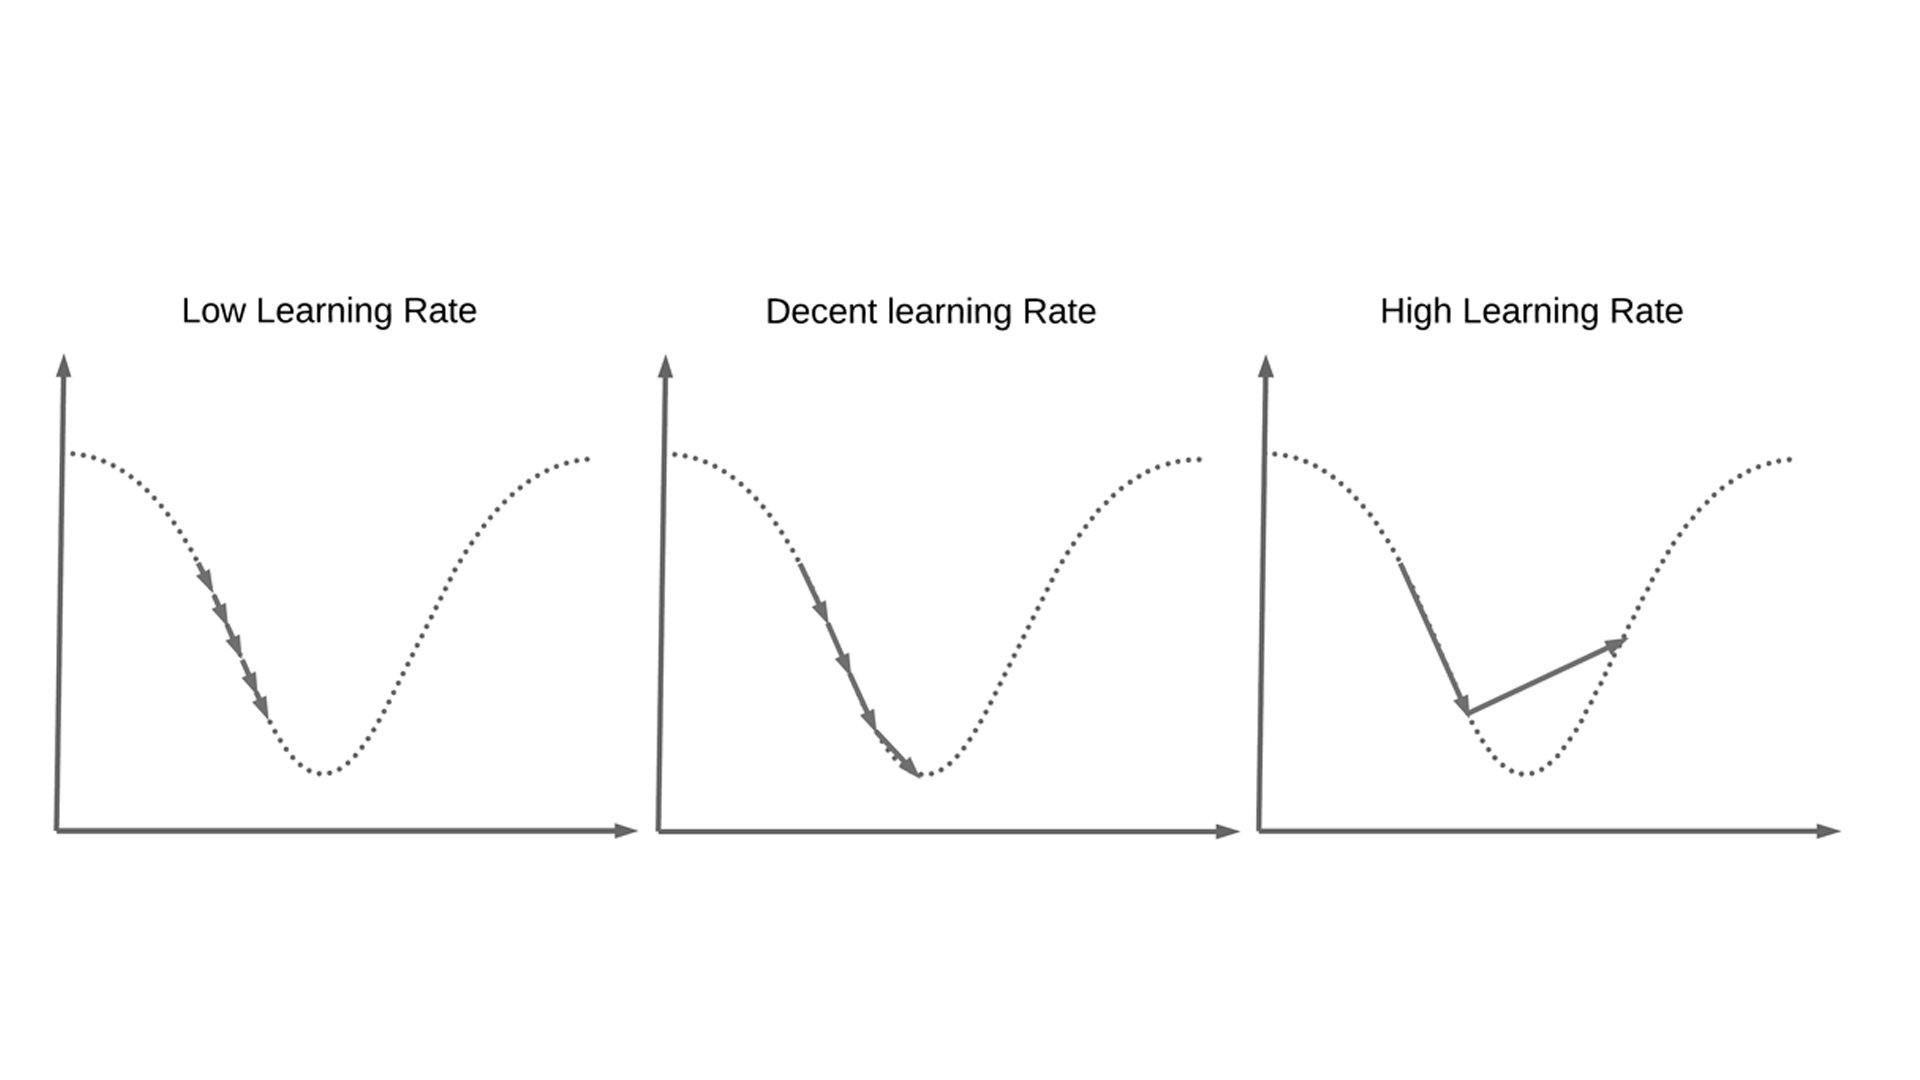
\includegraphics[width=400pt, keepaspectratio]{images/lrate}
    \caption[Einstellen der Lernrate]{Sehr gut erkennbar sind die Iterationen: Wenn die Lernrate richtig gewählt ist, dann erreicht sie das Minimun schneller.}
\end{figure}
Trotz des Algorithmus kann die Berechnung immer noch nicht effizient genug sein, denn wenn als
Beispiel der Datensatz von MNIST verwendet wird, dann müssen für alle 70000 Bilder die Gradienten berechnet werden. Diese Zeit kann erspart werden,
indem nicht für alle Bilder den Gradient berechnen werden müssen. Als Beispiel soll nur der Gradient berechnet werden bei jedes 100. Bild. So werden die Gradienten statt
für 70000 Bilder, nur 700 Bilder berechnet. Die Antastung des Minimums ist nicht sehr präzise, aber dennoch aussagekräftig und zeitsparend. Die
Optimierung nennt sich Stochastisches Gradientenverfahren (SGD).
\subsubsection{Backpropagation}\label{back}
Um die Parameter zu aktualisieren muss der Wert $\frac{\partial C}{\partial w_{i}}$ berechnet werden. Mithilfe der Backpropagation kann dieser Wert
berechnet werden, indem rückwärts gegangen wird vom FNN.\@ Als Beispiel wird ein FNN dargestellt mit drei Schichten. Für die Verlustfunktion soll der
Cross Entropy verwendet werden. Ziel ist es den Parameter $w_{2,3}^{(2,1)}$ zu aktualisieren, weshalb $\frac{\partial C}{\partial w_{2,3}^{(2,1)}}$ gesucht ist.
\begin{figure}[h]
    \centering
    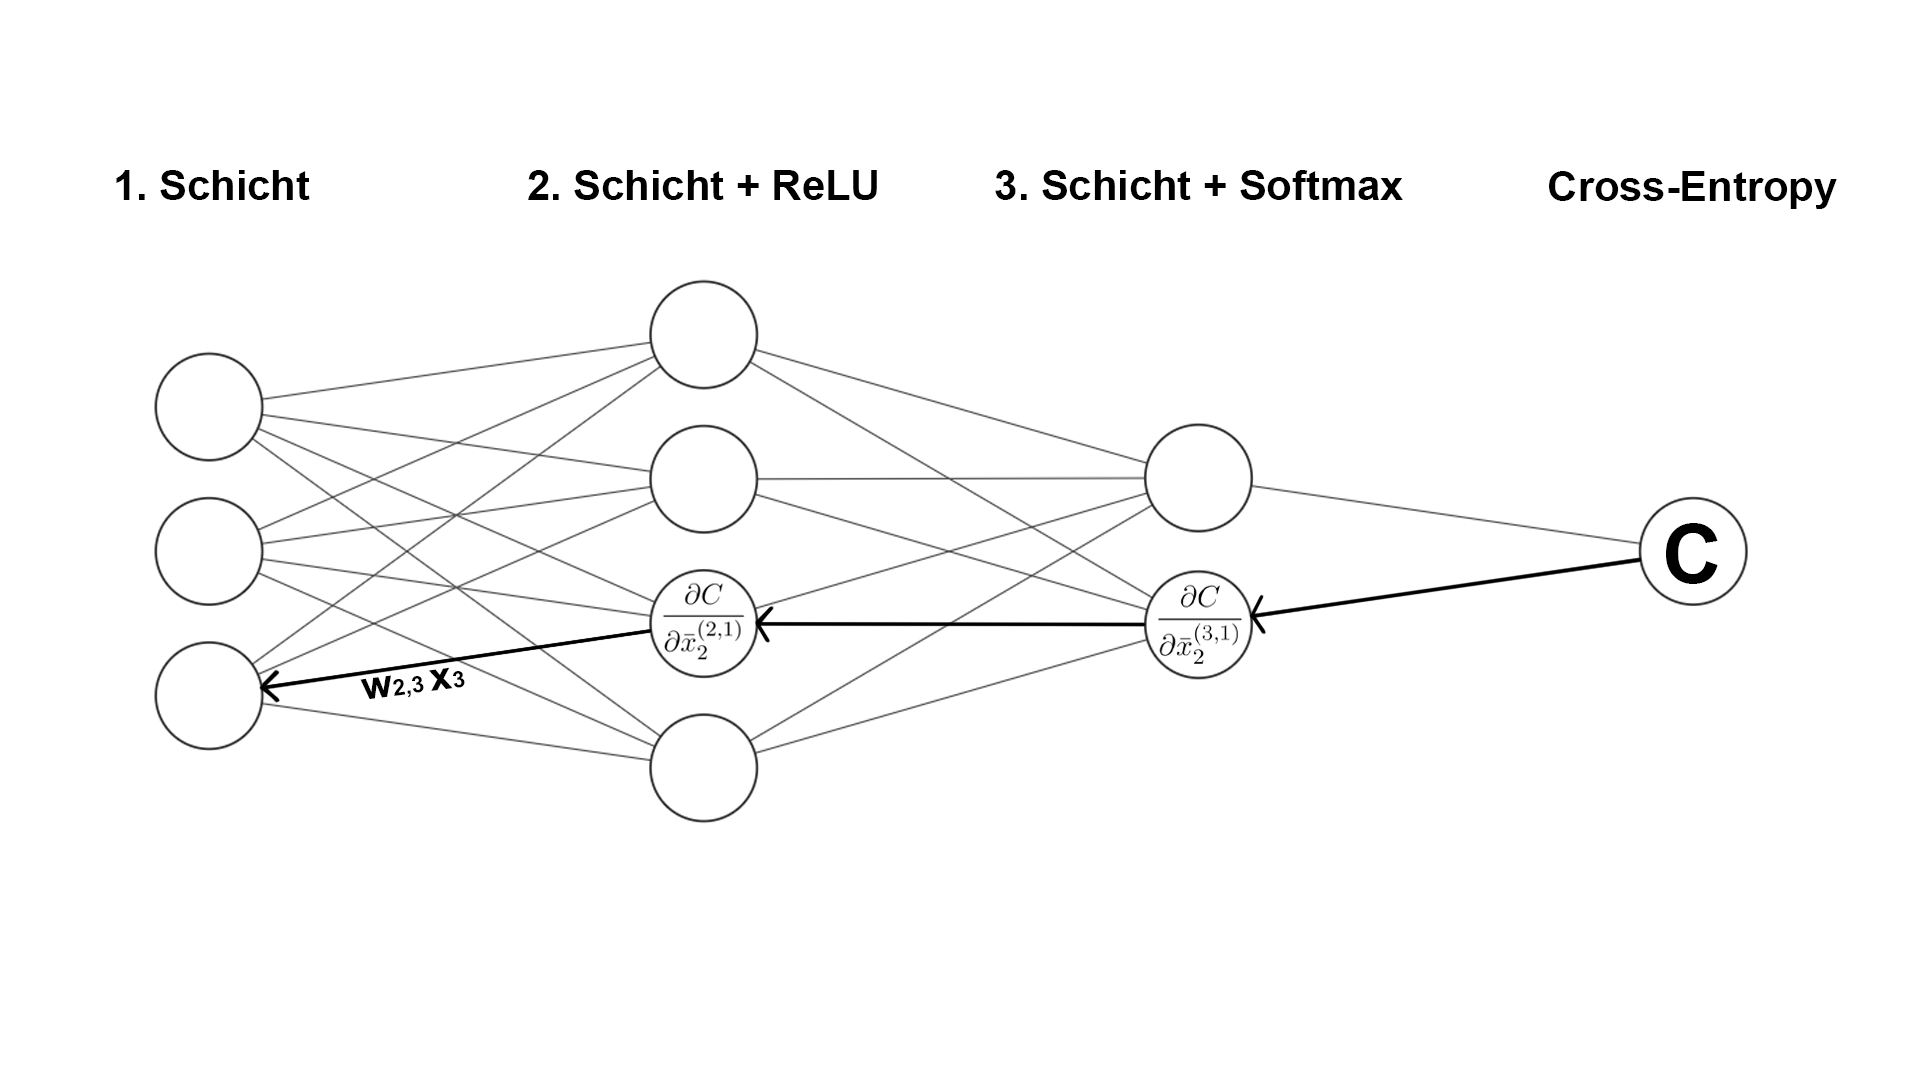
\includegraphics[width=400pt, keepaspectratio]{images/beispiel}
    \caption[Beispiel eines FNNs]{Der Pfad von der Verlustfunktion zum Parameter $w_{2,3}^{(2,1)}$. Dafür wird die Kettenregel angewendet, um die Abhängigkeit von $w_{2,3}^{(2,1)}$ zu berechnen.}
\end{figure}
Dafür wird angeschaut, wie die Verlustfunktion $C$ von $w_{2,3}^{(2,1)}$ abhängt.
Da die Werte bei jeder Schicht weitergegeben wurde, kann die Kettenregel angewendet werden:
\begin{equation}
    \frac{\partial C}{\partial w_{2,3}^{(2,1)}} = \frac{\partial C}{\partial x_2^{(3,1)}} \frac{\partial x_2^{(3,1)}}{\partial \bar{x}_2^{(3,1)}}
    \frac{\partial \bar{x}_2^{(3,1)}}{\partial x_2^{(2,1)}} \frac{\partial x_2^{(2,1)}}{\partial \bar{x}_2^{(2,1)}}
    \frac{\partial \bar{x}_2^{(2,1)}}{\partial w_{2,3}^{(2,1)}}
\end{equation}
Dies kann abgekürzt werden mit:
\begin{equation}\label{einfacher}
    \frac{\partial C}{\partial w_{2,3}^{(2,1)}} = \frac{\partial C}{\partial \bar{x}_2^{(2,1)}} \frac{\partial \bar{x}_2^{(2,1)}}{\partial w_{2,3}^{(2,1)}} \stackrel{(\ref{w})}{=} \frac{\partial C}{\partial \bar{x}_2^{(2,1)}} x_3^{(1,1)}
\end{equation}
Die Gleichung~\ref{einfacher} ist für die Umsetzung deutlich angenehmer, da der Wert $\frac{\partial C}{\partial \bar{x}_2^{(2,1)}}$ von der nächsten Schicht
schon berechnet wurde. Dies bedeutet, dass nur der Wert $\frac{\partial \bar{x}_2^{(2,1)}}{\partial w_{2,3}^{(2,1)}}$ berechnet werden muss.

\section{Umsetzung}
Zuerst braucht es eine Struktur für das CNN.\@ Dafür wird eine Klasse Layer erstellt, die als Objekt angesehen werden soll. Dabei soll die Layer folgende
Eigenschaften besitzen: Eine Eingabe und eine Ausgabe. Außerdem wird eine neue Klasse DenseLayer erstellt, die diese Eigenschaften der Klasse Layer erben.
Der DenseLayer soll die Schichten im FNN darstellen und die Parameter $w$ und $b$ als Variablen annehmen können. Weitere Klassen, wie Schichten für die
Feature Extraction oder Aktivierungsfunktion und Verlustfunktion müssen erstellt werden. Vorteil an der Programmierung sind die Open Source Pakete, die das
Internet anbietet. So müssen nicht die einzelne Elemente der Vektoren ausgerechnet werden, sondern kann alle Elemente des Verktors aufeinmal berechnen.
Auch muss der Lernprozess programmiert werden, indem das Netzwerk durchläuft. Die Anzahl der Durchläufe des Netzwerkes kann bestimmt werden.
Diese nennt sich auch Epochen. Am Ende werden verschiedene Diagramme generiert, die für die Analyse der KI nutzlich sein könnten.
Mehr dazu im Kapitel \nameref{auswertung}. Für die Architektur des Netzwerkes werden mehrere 2D Konvolutionsschichten, sowie Max Pooling Schichten angesetzt.
Der Aufbau ist gut im Abbild 12 zu erkennen.
\begin{figure}[h]
    \centering
    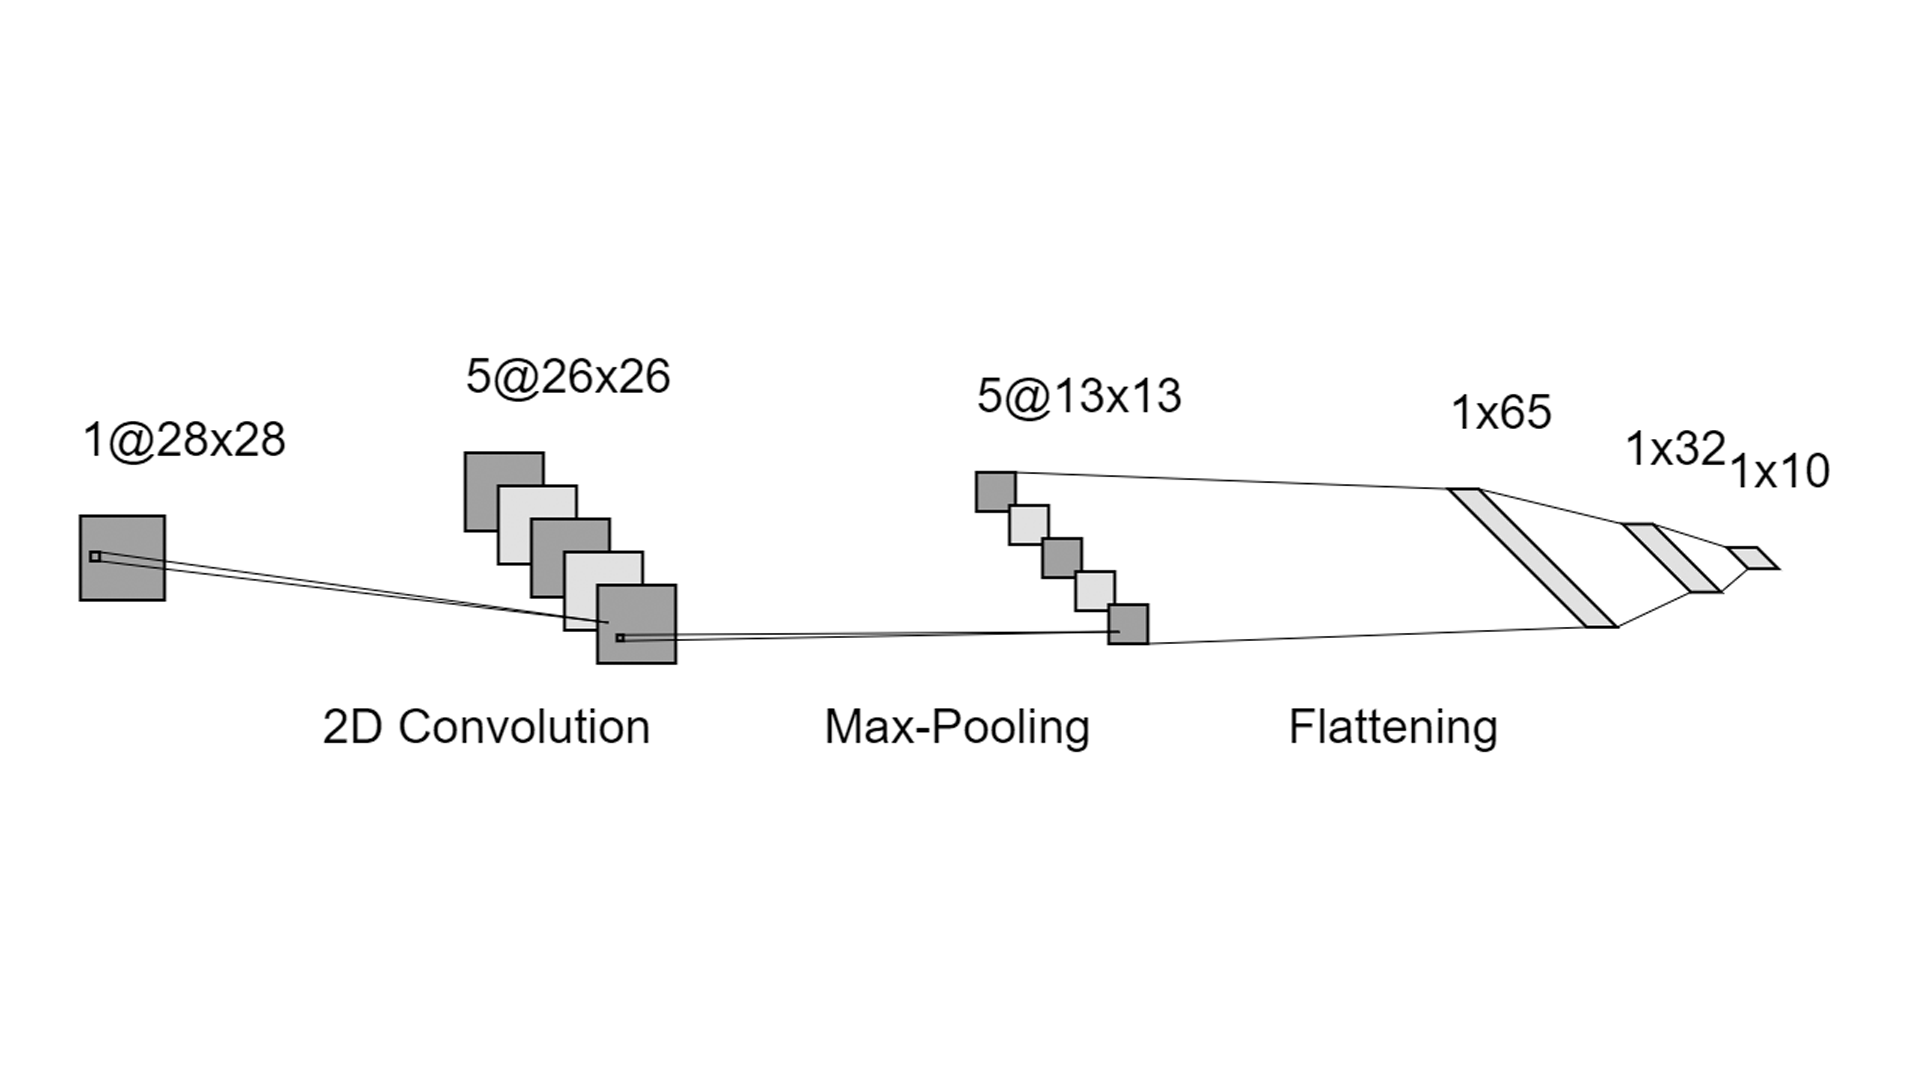
\includegraphics[width=400pt, keepaspectratio]{images/cnn}
    \caption[Architektur eines CNNs]{Insgesamt 8 Schichten mit gestapelten Operationen, wie die 2D Konvolution, oder der Max Pooling.
    Die Anzahl der Ausgabeschicht liegt bei 10, für die einzelnen Ziffern von 0-9.}
\end{figure}
Nach der Max-Pooling Schicht wird das zum Vektor abgeflacht und mit zwei weiteren neuronale Schichten verbaut.
Mit dem Netzwerk wird die Facharbeit die KI trainieren.

\subsection{Werkzeuge}
Für die Umsetzung wird die Programmiersprache Python verwendet, denn Python wird in der Praxis größtenteils für Data Science verwendet.
Python wird dafür verwendet, weil sie sehr gute Open Source Pakete besitzt. Dabei spielen zwei Pakete eine wichtige Rolle für die Umsetzung:
NumPy und Matplotlib. NumPy ist ein Paket für Vektor- und Matrizenberechnungen und berechnet die Werte effizienter als Python selbst. Außerdem
bietet sie sehr viele Operationen an, die für die KI notwendig sind. Der Matplotlib ist für die Visualisierung der Bilder, sowie die Filter von der
Feature Extraction zuständig. Sie hilft den Nutzer die KI besser zu verstehen und nachzuvollziehen.

\subsection{Trainingsphase}
Bevor der Ablauf in der Trainingsphase erklärt wird, wird der Datensatz in 3 Teilen aufgespalten: Die Trainingsdaten, die Validierungsdaten
und die Testdaten. Das Verhältnis der Verteilung kann unterschiedlich sein. Meistens sind sie in 50/30/20 aufgeteilt.
Für die Trainingsphase wird erstmal nur die Trainingsdaten und die Validierungsdaten verwendet.
Bevor die Trainingsphase gestartet wird, werden für alle verstellbare Parameter $w$, $b$ und $k$ zufällige Werte gegeben über
die Gauß-Verteilung. Zuerst wird ein zufälliges erstes Bild aus den Trainingsdaten in die Eingabeschicht weitergeleitet.
Bis zur Ausgabeschicht berechnet die KI die entsprechende Vorhersage. Mit der Vorhersage wird die Fehlerabweichung mit dem richtigen
Ergebnis mithilfe der Verlustfunktion berechnet. Die Parameter werden dann durch den SGD optimiert mithilfe von Backpropagation.
Danach wird das nächstes zufälliges Bild ausgewählt und die Schritte werden wiederholt. Dies gilt solange, bis der alle Bilder aus
den Trainingsdaten einmal vorgekommen sind. Zuletzt werden die Bilder aus den Validierungsdaten
in die Eingabeschicht weitergeleitet und die KI soll die Zahl vorhersagen. Der Unterschied ist aber, dass die Parameter nicht optimiert werden
und dass sozusagen die KI nur getestet wird. Die erste Epoche endet somit und die zweite Epoche beginnt. Sie wiederholt die oben genannten Schritte,
wie in der ersten Epoche. Der Vorteil ist aber, dass sie mit den verbesserten Parameter weiterrechnet. Die Anzahl der Epochen, die durchgangen
werden sollen kann selber bestimmt werden. Für die Facharbeit wurde die Epoche auf 200 gesetzt. Am Ende der Trainingsphase wird ein Diagramm
angezeigt, die für den Kapitel Auswertung eine wichtige Rolle spielen.

\subsection{Auswertung}\label{auswertung}
Manchmal kann bei schlecht ausgewählte Strukur des Netzwerkes die Vorhersehbarkeit der KI beeinträchtigen.
Dafür werden zwei neue Begriffe definiert: Überfittung (Overfitting) und Unterfittung (Underfitting).
Als Beispiel werden 3 verschiedene Regressionen verwendet:
\begin{figure}[h]
    \centering
    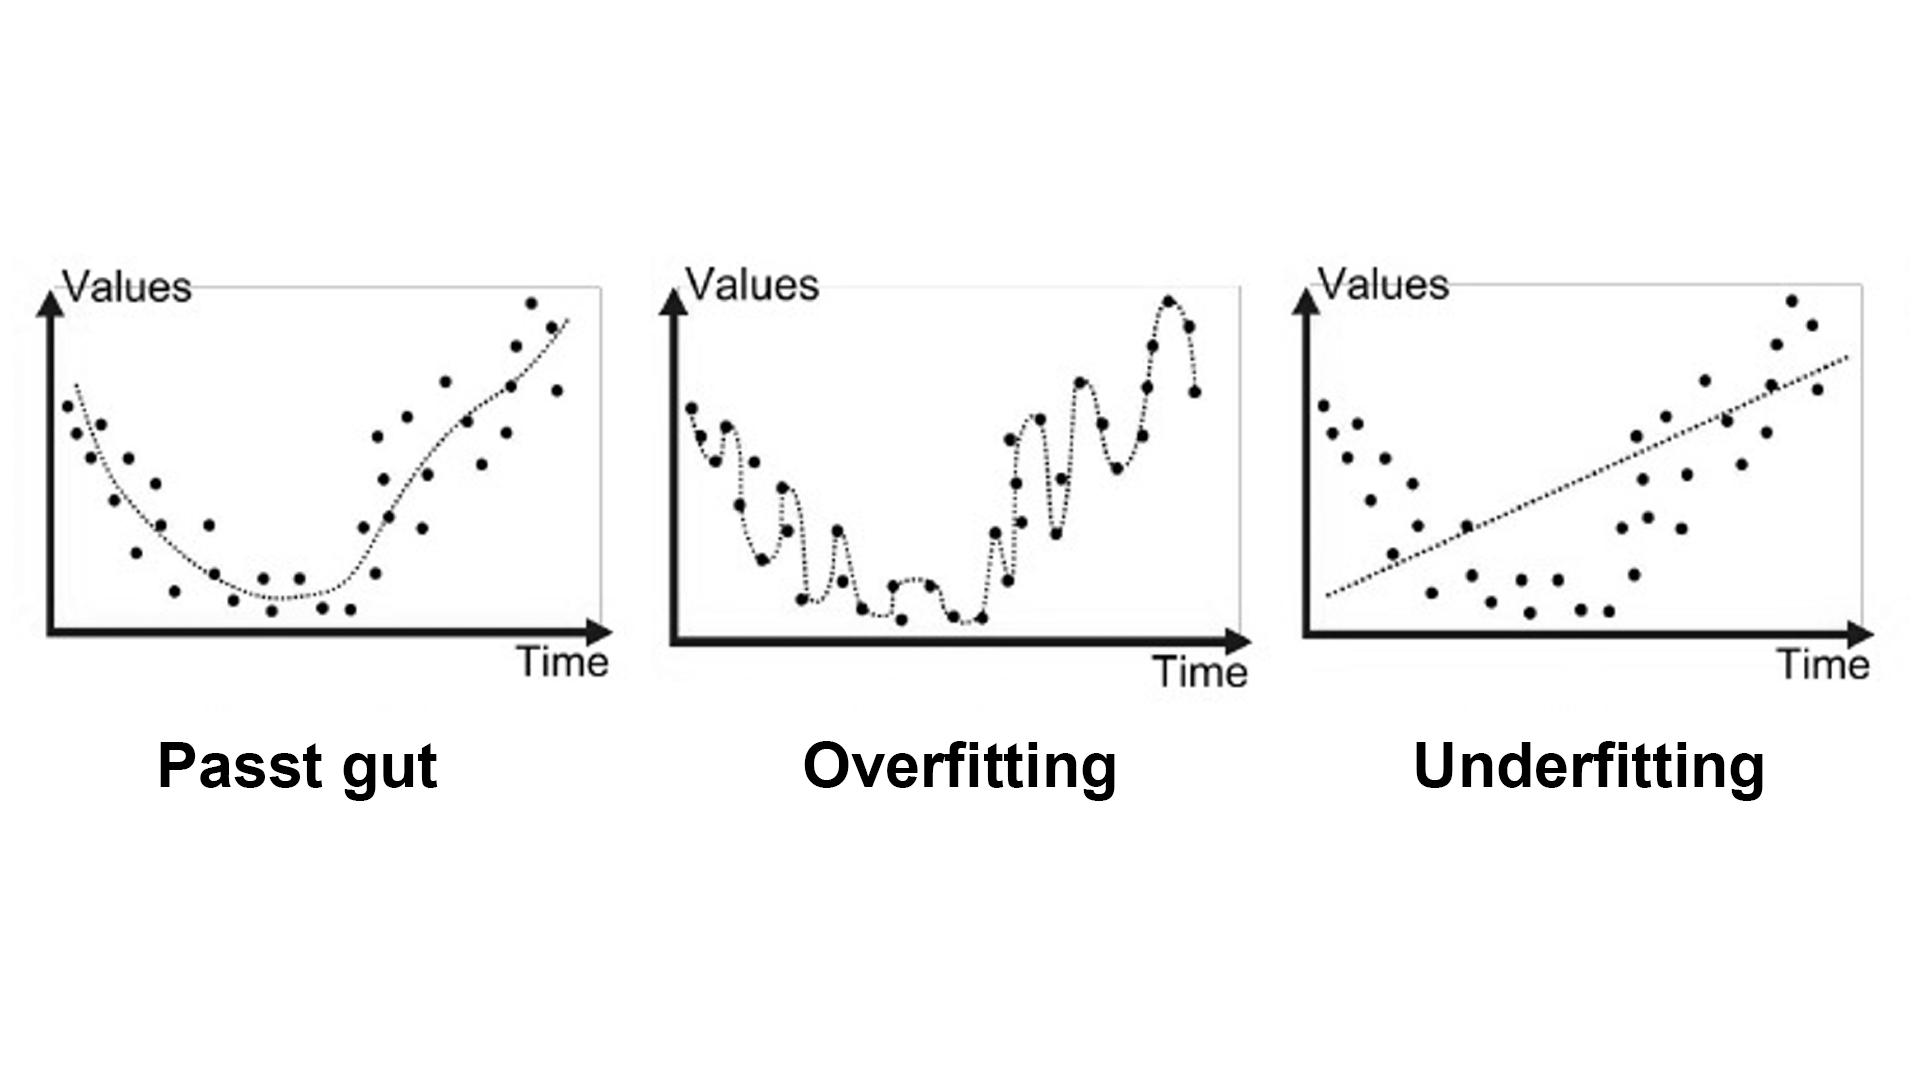
\includegraphics[width=330pt, keepaspectratio]{images/overfitting}
    \caption[Overfitting und Underfitting]{Die Regressionen werden als Beispiel mit Overfitting und Underfitting dargestellt.}
\end{figure}
Von den 3 Regressionen ist die erste Regression gut gewählt, denn sie verläuft nicht allzu perfekt in den Punkten. Trotzdem sind die
Abweichungen gering. Bei der zweite Regression wird Overfitting erkannt, denn sie verläuft zu perfekt in den Punkten, doch wenn
ein neuer unbekannter Punkte eingefügt wird, dann kann die Regression zu falsche Ergebnisse führen. Das Gegenteil davon ist Underfitting
bei der dritten Regression. Hier wird deutlich gezeigt, dass die Abweichungen zu hoch sind, weil die Regression linear ist.
Dies kann mit der Trainingsphase bei der KI übertragen werden, denn die KI soll sich nicht zu sehr auf die Trainingsdaten gewöhnen,
sondern auch von unbekannten Daten gut vorhersagen. Deswegen spielen die Validierungsdaten eine wichtige Rolle, um gegen Overfitting
und Underfitting vorzugehen. Um zu sagen, wie gut eine KI vorhersagen kann werden sogenannte Metriken verwendet. Metriken sind Bewertungskriterien für die KI,
wie gut sie vorhersagen kann. Eine, die für die Facharbeit genommen wird ist die Genauigkeit (Accuracy). Sie lässt sich folgendermaßen
berechnen:
\begin{equation}
    \frac{\text{Anzahl der richtig vorhergesagten Bildern}}{\text{Anzahl der Gesamtbildern}}
\end{equation}
Das Diagramm, das in Kapitel Trainingsphase erwähnt wurde, ist ein Epoche-Accuracy Diagramm und sieht folgendermaßen aus nachdem die Trainingsphase
beendet wurde:
\begin{figure}[h]
    \centering
    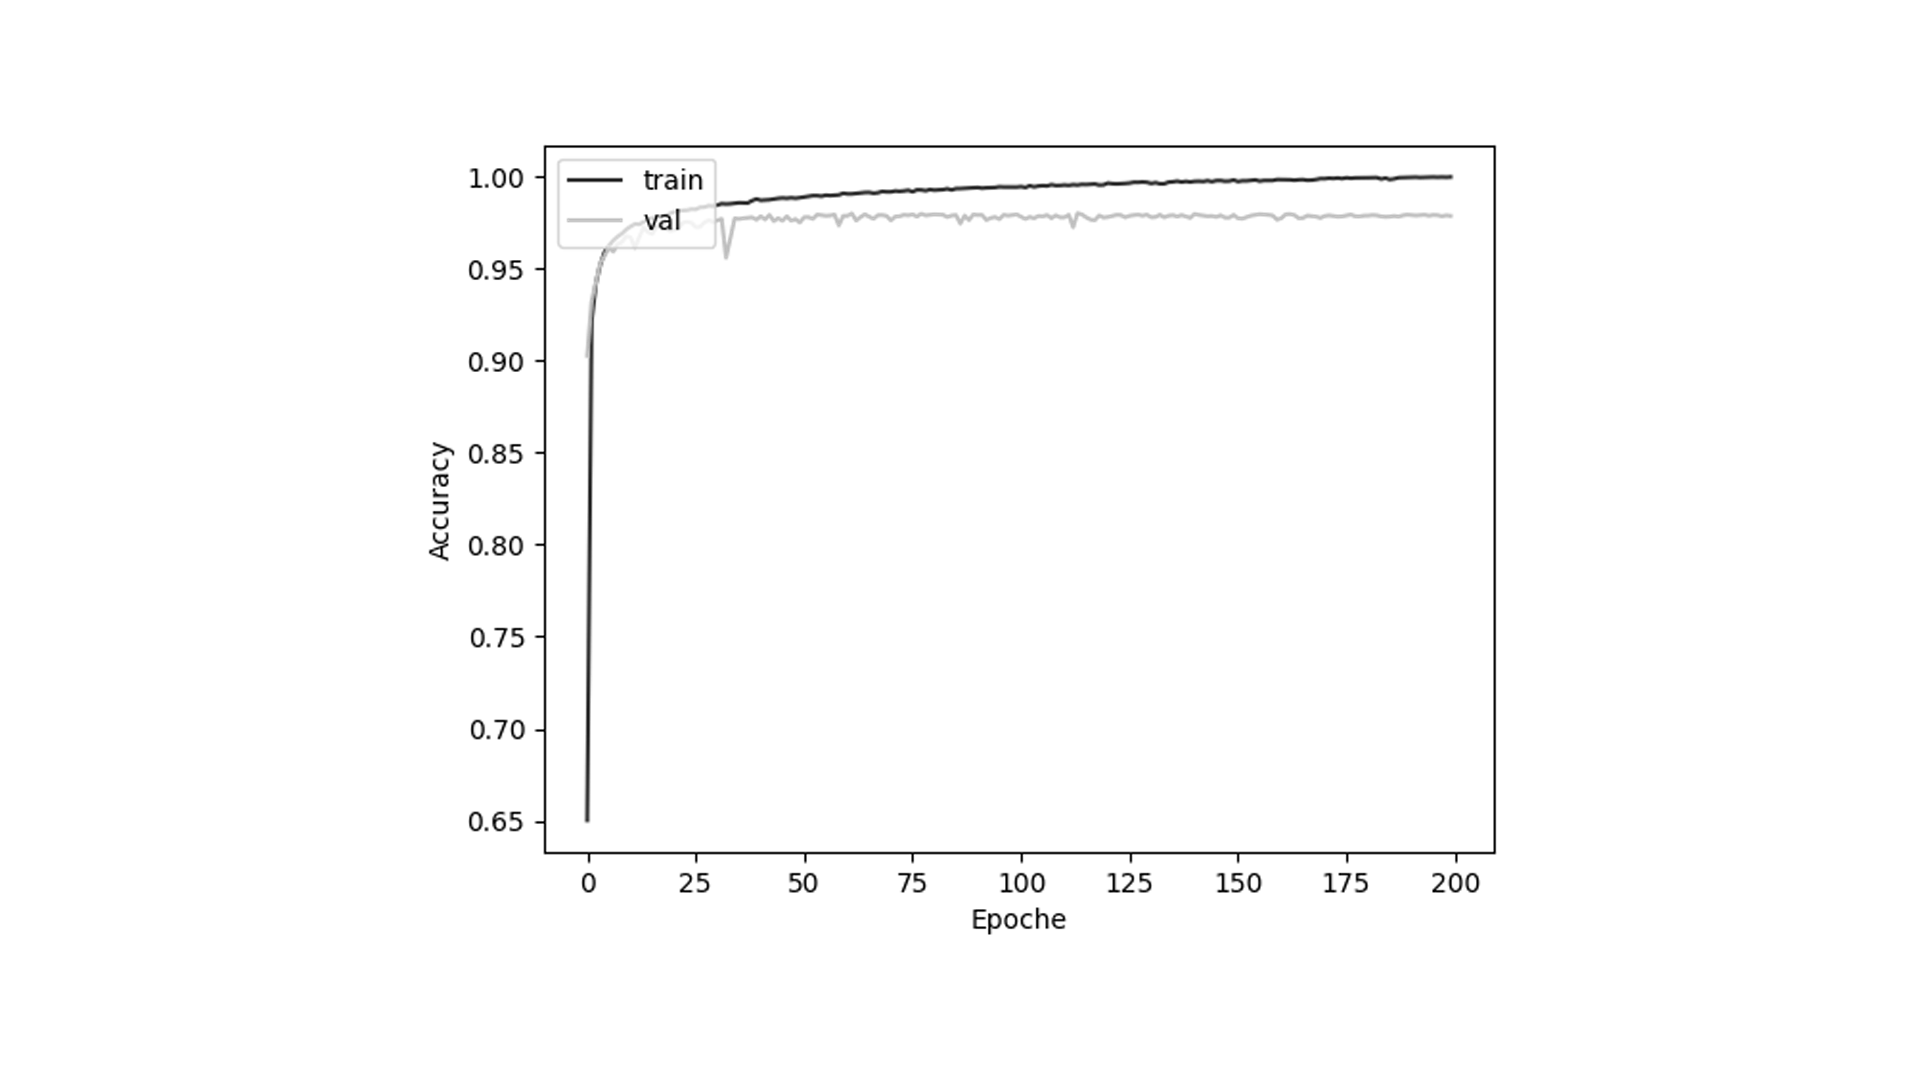
\includegraphics[width=340pt, keepaspectratio]{images/accuracydiagram}
    \caption[Epoche-Accuracy Diagramm]{Epoche-Accuracy Diagramm mit den Werten der Testdaten und der Validierungsdaten. Der Abstand vergrößert sich,
    die KI fängt an zu überfitten.}
\end{figure}
Hier ist gut zu sehen, dass während die Accuracy der Trainingsdaten nach oben steigt die Validierungsdaten der KI konstant bleibt. Die Abstand zwischen den
beiden Werten nimmt zu. Dies deutet auf Overfitting hin und kann durch früheres aufhören verhindert werden. Für diesen Fall reichen
75 Epochen. Zum Schluss werden die Testdaten auch in das Netzwerk reingeschickt und versucht vorherzusagen. Unterschied zwischen den Validierungsdaten
und Testdaten ist, dass die Testdaten noch keinen Kontakt mit der KI hatten, sodass die KI getestet werden kann.
Nach der Durchführung liegt der Accuracy Wert der Testdaten bei 98,17\%.

\section{Schlussfolgerung}


\newpage
\nolinenumbers{}
%\section{Literaturverzeichnis} wenn Literaturverzeichnis dabei sein muss in der Gliederung
{
%\renewcommand{\section}[2]{}
\renewcommand\refname{Literaturverzeichnis}
\hypersetup{linkcolor=red}
\renewcommand\UrlFont{\color{black}\normalfont}
\begin{thebibliography}{15}
    \bibitem{useofki}

    Europäisches Parlament: Was ist künstliche Intelligenz und wie wird sie genutzt?. 2021. Stand: 24.11.2022.
    \url{https://www.europarl.europa.eu/news/de/headlines/society/20200827STO85804/was-ist-kunstliche-intelligenz-und-wie-wird-sie-genutzt}
    [\ref{1}]
    
    \bibitem{weakki}
    Uni Oldenburg: Schwache KI und Starke KI.\@ 2008/2009. Stand: 24.11.2022.
    \url{http://www.informatik.uni-oldenburg.de/~iug08/ki/Grundlagen_Starke_KI_vs._Schwache_KI.html}
    [\ref{2}]

    \bibitem{mnist}
    Yann LeCun, Corinna Cortes, Christopher J.C. Burges: THE MNIST DATABASE of handwritten digits. Stand: 24.11.2022.
    \url{http://yann.lecun.com/exdb/mnist/}
    %[\ref{3}]

    \bibitem{wasistki}
    Bundesministerium für Wirtschaft und Energie: Zur Diskussion der Effekte Künstlicher Intelligenz in der wirtschaftswissenschaftlichen Literatur. 2018. Stand: 24.11.2022.
    \url{https://www.bmwk.de/Redaktion/DE/Downloads/Diskussionspapiere/20190205-diskussionspapier-effekte-kuenstlicher-intelligenz-in-der-wirtschaftswissenschaftlichen-literatur.pdf?__blob=publicationFile&v=6}
    %[\ref{4}]

    \bibitem{learnneuralnetwork}
    Michael Nielsen: Neural Network and Deep Learning. 2019. Stand: 24.11.2022.
    \url{http://neuralnetworksanddeeplearning.com/}
    %[\ref{5}][\ref{9}]

    \bibitem{typeofneural}
    My Great Learning: Types of Neural Networks and Definition of Neural Network. 2022. Stand: 24.11.2022.
    \url{https://www.mygreatlearning.com/blog/types-of-neural-networks/}
    %[\ref{6}]

    \bibitem{book}
    Chi Nhan Nguyen, Oliver Zeigermann: Machine Learning kurz \& gut O’Reillys Taschenbibliothek. 2. Auflage. 2021
    %[\ref{7}]

    \bibitem{optimizer}
    Musstafa: Optimizers in Deep Learning. 2021. Stand 24.11.2022.
    \url{https://medium.com/mlearning-ai/optimizers-in-deep-learning-7bf81fed78a0}
    %[\ref{8}]

    \bibitem{github}
    Bui Anh Minh Leon Phan: handwrittenDigits. 2022. Stand: 24.11.2022.
    \url{https://github.com/xXChezyXx/handwrittenDigits}
    %[\ref{10}]

    \bibitem{bwki}
    Bundeswettbewerb KI:\@ Künstliche Intelligenz. 2022. Stand: 24.11.2022.
    \url{https://www.bw-ki.de/}
    %[\ref{11}]

\end{thebibliography}
}
\newpage
\section*{Schülererklärung}
Hiermit erkläre ich, dass ich die vorliegende Seminarfacharbeit selbstständig angefertigt,
keine anderen als die angegebenen Hilfsmittel benutzt und die Stellen der Seminarfacharbeit,
die im Wortlaut oder im wesentlichen Inhalt aus anderen Werken entnommen wurden,
mit genauer Quellenangabe kenntlich gemacht habe.

\end{document}